%========================================================
%% TITLE	An Introduction to Finite Element Method - main.tex
%% DATE	
%%          - 21/06/2026 (version 1)

%% AUTHOR	BINGHUAN W LI (Dept. Chemical Eng/Bio Eng, Imperial)

%% compiled in XeLaTeX with Tex Live version 2023.

%% This work is licensed under a Creative Commons Attribution-NonCommercial 4.0 International License.
%========================================================
\documentclass[12pt, a4paper]{article}
\usepackage[margin=1.8cm]{geometry}
\usepackage{amsfonts, amsmath, amssymb, cancel}
\numberwithin{equation}{section}
\usepackage{booktabs}
\usepackage{enumitem}

\usepackage[export]{adjustbox}
\usepackage{appendix}
\usepackage{fontspec}
    \setmainfont{XITS}
\usepackage[bold-style=ISO]{unicode-math}
    \setmathfont{XITS Math}

\usepackage{xcolor}
    \definecolor{linkcolour}{rgb}{0,0.2,0.6}

\usepackage{titling}
    \setlength{\droptitle}{-3em}
    
\usepackage{hyperref}
\hypersetup{
    colorlinks,
    breaklinks,
    urlcolor=linkcolour,
    linkcolor=black,
    citecolor=black,
    pdftitle={An Introduction to the Finite Element Method},
    pdfauthor={Li, Binghuan},
    }

\usepackage[rightcaption]{sidecap} % Options: rightcaption, leftcaption, raggedright, raggedleft
\sidecaptionvpos{figure}{b} % Aligns caption vertically: m (middle), t (top), or b (bottom)
\usepackage{graphicx, float}


\usepackage{imakeidx}
\makeindex

\usepackage{biblatex}
\addbibresource{assets/refs.bib}

\usepackage{fontawesome}

% pseudo code listing
\usepackage{algorithm}
\usepackage{algpseudocode}

\usepackage{mdframed}
\usepackage[breakable]{tcolorbox}
\usepackage{tikz}
\usetikzlibrary{shapes.geometric, arrows}
\tikzstyle{process} = [rectangle, minimum width=3cm, minimum height=1cm, text centered, draw=black]
\tikzstyle{arrow} = [thick,->,>=stealth]

\setlength\parindent{0pt}
\linespread{1.15}
\graphicspath{{./figures/}}

%========================================================
%% TITLE	An Introduction to Finite Element Method - command_lst.tex
%% DATE	
%%          - 21/06/2026 (version 1)

%% AUTHOR	BINGHUAN W LI (Dept. Chemical Eng/Bio Eng, Imperial)

%% compiled in XeLaTeX with Tex Live version 2023.

%% This work is licensed under a Creative Commons Attribution-NonCommercial 4.0 International License.
%========================================================

% B, D, shape function matrix
\newcommand{\B}[0]{[\mathbf{B}]}
\newcommand{\D}[0]{[\mathbf{D}]}
\newcommand{\N}[0]{[\mathbf{N}]}

\newcommand{\vel}[0]{\dot{\mathbf{u}}}
\newcommand{\acc}[0]{\ddot{\mathbf{u}}}

% stress
% \stress is the Voigt stress vector
\newcommand{\stress}[0]{\{\boldsymbol{\sigma}\}}

% Continuum stress tensors: no curly braces
\newcommand{\bS}[0]{\mathbf{S}}
\newcommand{\bP}[0]{\mathbf{P}}

% strain
% \strain is the Voigt strain vector
\newcommand{\strain}[0]{\{\boldsymbol{\varepsilon}\}}

% Continuum strain/deformation tensors: no curly braces
\newcommand{\bE}[0]{\mathbf{E}}
\newcommand{\be}[0]{\mathbf{e}}
\newcommand{\bb}[0]{\mathbf{b}}
\newcommand{\bC}[0]{\mathbf{C}}

% FEM nodal displacement vector
\newcommand{\bU}[0]{\{\mathbf{U}\}}

% rot
\newcommand{\bR}[0]{\mathbf{R}}

% identity tensor / matrix
% Use this as the continuum identity tensor.
% If you specifically need the matrix representation, [\mathbf{I}] is also acceptable,
% but avoid mixing both in the same equation.
\newcommand{\II}[0]{\mathbf{I}}

% element and global stiffness matrix
\newcommand{\kloc}[0]{[\mathbf{k}^e]}
\newcommand{\kglob}[0]{[\mathbf{K}]}

% element and global force vector
\newcommand{\fglob}[0]{\{\mathbf{f}_{\mathrm{ext}}\}}
\newcommand{\floc}[0]{\{\mathbf{f}_{\mathrm{ext}}^e\}}

% plain bold symbols / fallback aliases
\newcommand{\bB}[0]{\mathbf{B}}

\newcommand{\bd}[0]{\mathbf{d}}
\newcommand{\bD}[0]{\mathbf{D}}
\newcommand{\bff}[0]{\mathbf{f}}
\newcommand{\bF}[0]{\mathbf{F}}
\newcommand{\bk}[0]{\mathbf{k}}
\newcommand{\bK}[0]{\mathbf{K}}
\newcommand{\bM}[0]{\mathbf{M}}
\newcommand{\bN}[0]{\mathbf{N}}
\newcommand{\bt}[0]{\mathbf{t}}

% physical displacement vector field
\newcommand{\bu}{\mathbf{u}}
% \newcommand{\bU}[0]{\{\mathbf{U}\}}

% example block
\usepackage{xcolor}
\newtcolorbox[auto counter]{example}[2][]{
   boxrule=0pt,
   coltitle=black,
   sharp corners,
   breakable, 
   title={\color{white}\textbf{Example~\thetcbcounter: \ #1 #2}}
   }
\newtcolorbox[auto counter]{remark}[2][]{
   boxrule=0pt,
   coltitle=black,
   sharp corners,
   breakable, 
   title={\color{white}\textbf{Remark~\thetcbcounter: \ #1 #2}}
   }
%==============================================================
%==============================================================
\title{\textbf{An Introduction to the Finite Element Method}}
\author{\textbf{Binghuan Li} \\
        Department of Bioengineering / Chemical Engineering \\ Imperial College London \\
        \texttt{binghuan.li19@imperial.ac.uk}
        }
\date{Version 1.0, Last Update: \today}

\begin{document}
%==============================================================
\maketitle
\tableofcontents
%==============================================================
\section*{Preface}
%==============================================================
This noteset provides a concise summary of the theoretical introduction to the Finite Element Method, with particular emphasis on mechanical stress analysis.\\

The main sections of these notes were inspired by the skeleton of the course materials on \textit{Biomedical Advanced and Computational Stress Analysis} by Professor Spyros Masouros, and \textit{Computational Continuum Mechanics} by Professor Daniel Balint, both at Imperial College London. The notes on the topic of kinematics also integrated insights from \textit{Nonlinear solid mechanics: a continuum approach for engineering science} by Professor Gerhard Holzapfel.\\

It should be noted, however, that this is a redacted version of FEM notes. Calculation examples will be provided in the subsequent version updates; practical examples can be prepared upon request. Advanced concepts, including (but not limited to) the nonlinear finite element method, contact, time integration, and weighted residual method, variational calculus, were truncated for simplicity and clarity of these notes. \\

\faGithub \ The \LaTeX \ files are now accessible on my \href{https://github.com/binghuan-li/Notes-and-Formula-Sheets}{\texttt{GitHub} repository}. I hope it helps. The technical content of these notes was prepared by the author, without relying on AI-generated material; please report any typos, errors, and inconsistencies found to \href{mailto:binghuan.li19@imperial.ac.uk}{\texttt{binghuan.li19@imperial.ac.uk}}. \\

\begin{flushright}
    July 2026, London
\end{flushright}

% BY-CC
\vfill    
\begin{figure}[H]
    \includegraphics[right]{by-nc.eps}
\end{figure}
\textit{This work is licensed under a Creative Commons Attribution-NonCommercial 4.0 International License.}


%==============================================================
\newpage
\section{Introduction}
%==============================================================

The finite element method (FEM) is an approximate numerical method to solve problems in engineering and mathematical sciences. In stress analysis, FEM helps predict how a structure or material deforms, strains, and carries stress under given loads and boundary conditions. \\

As shown in Figure~\ref{fig:FEA_logics}, the basic idea of FEM is to:
\begin{itemize}
    \item define the geometry of the problem,
    \item assign material properties,
    \item apply loads and boundary conditions,
    \item divide the geometry into smaller elements, called a mesh,
    \item solve for the unknown nodal displacements,
    \item calculate the resulting strains and stresses.
\end{itemize}

\begin{figure}[ht!]
\centering
\begin{tikzpicture}[node distance=1cm]
    \node (geometry) [process] {Geometry};
    \node (mesh) [process, below of=geometry, yshift=-0.5cm] {Mesh};
    \node (boundary) [process, left of=mesh, xshift=-3cm] {Boundary conditions};
    \node (material) [process, right of=mesh, xshift=3cm] {Material properties};
    \node (continuum) [process, below of=mesh, yshift=-0.5cm, draw=blue, ultra thick] {Solve continuum mechanics};
    \node (mechanical) [process, below of=continuum, yshift=-0.5cm, draw=green, ultra thick] {Mechanical Behaviour};
    \draw [arrow] (geometry) -- (mesh);
    \draw [arrow] (mesh) -- (continuum);
    \draw [arrow] (boundary) -- (continuum);
    \draw [arrow] (material) -- (continuum);
    \draw [arrow] (continuum) -- (mechanical);
\end{tikzpicture}
\caption{Overview of the finite element analysis logics}
\label{fig:FEA_logics}
\end{figure}

In this way, FEM connects continuum mechanics theory with practical computational analysis. Instead of solving the entire body exactly, the method approximates the behaviour of each small element and assembles them into a complete model of the structure. 

\paragraph{Notes structure} The following chapters will introduce the main concepts needed to understand finite element analysis:
\begin{itemize}
    \item \textbf{Section 2} introduces the linear finite element method, including stress-strain relations, the constitutive matrix, the general FEA solution procedure, and the strain–displacement matrix.

    \item \textbf{Section 3} explains element-level computations, including shape functions, element mapping, Gaussian quadrature, and the evaluation of the element stiffness matrix.

    \item \textbf{Section 4} derives the element stiffness matrix using the principle of virtual work.

    \item \textbf{Section 5} extends the discussion towards continuum mechanics and nonlinear finite element methods, including deformation measures, strain energy functions, and hyperelastic materials.
\end{itemize}

Overall, these notes provide a compact introduction to FEM with an emphasis on its use in stress analysis.

\paragraph{Notations} Throughout these notes, the following notation convention is adopted. Curly braces, such as $\{\mathbf{U}\}$, $\{\boldsymbol{\varepsilon}\}$, and $\{\boldsymbol{\sigma}\}$, denote FEM column vectors. Square brackets, such as $[\mathbf{K}]$, $[\mathbf{B}]$, $[\mathbf{D}]$, and $[\mathbf{N}]$, denote FEM matrices. Bold symbols without brackets or braces, such as $\mathbf{F}$, $\mathbf{C}$, $\mathbf{b}$, $\mathbf{E}$, and $\boldsymbol{\sigma}$, denote tensors in continuum mechanics.


%==============================================================
\newpage
\section{Linear Finite Element Method}
%==============================================================

\subsection{Stress and Strain Measures}

\paragraph{The Stress and Strain Tensor}
Both the stress and strain tensors are the 2\textsuperscript{nd}-order tensors, which contain the information including the stress/strain magnitude, direction, and plane at which it acts. The \textit{Cauchy stress tensor}, $\boldsymbol{\sigma}$, is defined as
\begin{equation}
\label{eqn:Cauchy}
    \boldsymbol{\sigma} = 
    \begin{Bmatrix}
        \sigma_{xx} & \tau_{xy} & \tau_{xz} \\
        \tau_{yx} & \sigma_{yy} & \tau_{yz} \\
        \tau_{zx} & \tau_{zy} & \sigma_{zz} 
    \end{Bmatrix}
\end{equation}
where $\sigma_{ii}$ (the diagonal elements) denote normal stresses $\tau_{ij}$ (the off-diagonal elements) denote shear stresses. The first subscript indicates the plane where the stress is located, and the second subscript indicates the direction of the stress.\\

Similarly, the \textit{strain tensor}, $\boldsymbol{\varepsilon}$ is defined as
\begin{equation}
    \boldsymbol{\varepsilon} = 
    \begin{Bmatrix}
        \varepsilon_{xx} & \varepsilon_{xy} & \varepsilon_{xz} \\
        \varepsilon_{yx} & \varepsilon_{yy} & \varepsilon_{yz} \\
        \varepsilon_{zx} & \varepsilon_{zy} & \varepsilon_{zz} \\
    \end{Bmatrix}.
\end{equation}

By relation $\tau_{ij} = \tau_{ji}$ and $\varepsilon_{ij} = \varepsilon_{ji}$ (symmetry), the $3 \times 3$ stress and strain tensors can be simplified into column vectors with 6 independent elements, 
\begin{equation}
    \stress = 
    \begin{Bmatrix}
        \sigma_{x} \\
        \sigma_{y} \\
        \sigma_{z} \\
        \tau_{xy} \\
        \tau_{yz} \\
        \tau_{zx} 
    \end{Bmatrix},
    \quad \quad \quad
    \strain = 
    \begin{Bmatrix}
        \varepsilon_{x} \\
        \varepsilon_{y} \\
        \varepsilon_{z} \\
        \varepsilon_{xy} \\
        \varepsilon_{yz} \\
        \varepsilon_{zx} 
    \end{Bmatrix}
    \quad \text{or} \quad
    \strain = 
    \begin{Bmatrix}
        \varepsilon_{x} \\
        \varepsilon_{y} \\
        \varepsilon_{z} \\
        \gamma_{xy} \\
        \gamma_{yz} \\
        \gamma_{zx} 
    \end{Bmatrix}.
\end{equation}

Note that, in Voigt notation, engineering shear strains are used, where $\gamma_{ij} = 2\varepsilon_{ij}$.

\paragraph{Linear Elastic Materials}
An isotropic linear elastic material can be fully characterised by any two independent elastic constants.

\begin{itemize}
    \item The shear modulus, 
    \begin{equation}
        \mu = G = \frac{E}{2(1+\nu)},
    \end{equation}
    where $E$ denotes the Young's modulus, $\nu = -\dfrac{\text{lateral strain}}{\text{normal strain}}$ denotes the Poisson's ratio.

    \item The bulk modulus, $K$
    \begin{equation}
        K = \frac{E}{3(1-2\nu)},
    \end{equation}
    
    \item and the Lam\'e constants, $\lambda$ and $\mu$
    \begin{equation}
        \lambda = \frac{\nu E}{(1+\nu)(1-2\nu)}.
    \end{equation}
\end{itemize}
 
\paragraph{Stress-Strain Relation} There exist many formulations to characterise the isotropic linear elastic stress-strain relation. Using Lam\'e constants:

\begin{equation}
    \boldsymbol{\sigma} = \lambda \mathrm{tr} (\boldsymbol{\varepsilon}) \II + 2 \mu \boldsymbol{\varepsilon}
\end{equation}

Alternatively, the stress-strain relationship can be expressed using the generalised Hooke's Law
\begin{align}
    \varepsilon_x = \frac{1}{E} \left[ \sigma_x - \nu(\sigma_y + \sigma_z) \right]
    \quad & \quad
    \gamma_{xy} = \frac{\tau_{xy}}{G} = \frac{2(1+\nu)}{E} \tau_{xy} \\
    \varepsilon_y = \frac{1}{E} \left[ \sigma_y - \nu(\sigma_z + \sigma_x) \right]
    \quad & \quad
    \gamma_{yz} = \frac{\tau_{yz}}{G} = \frac{2(1+\nu)}{E} \tau_{yz} \\
    \varepsilon_z = \frac{1}{E} \left[ \sigma_z - \nu(\sigma_x + \sigma_y) \right]
    \quad & \quad
    \gamma_{zx} = \frac{\tau_{zx}}{G} = \frac{2(1+\nu)}{E} \tau_{zx}
\end{align}
Hence, one can express the stress $\sigma_i$ and $\tau_{ij}$ in terms of the strain
\begin{align}
\label{eqn:stress-strain_x}
    \sigma_x = \frac{E}{(1+\nu)} \varepsilon_x + \frac{E \nu}{(1+\nu) (1-2\nu)} \varepsilon_v,
    \quad & \quad
    \tau_{xy} = G \gamma_{xy} = 2G \varepsilon_{xy} \\
\label{eqn:stress-strain_y}
    \sigma_y = \frac{E}{(1+\nu)} \varepsilon_y + \frac{E \nu}{(1+\nu) (1-2\nu)} \varepsilon_v,
    \quad & \quad
    \tau_{yz} = G \gamma_{yz} = 2G \varepsilon_{yz} \\
\label{eqn:stress-strain_z}
    \sigma_z = \frac{E}{(1+\nu)} \varepsilon_z + \frac{E \nu}{(1+\nu) (1-2\nu)} \varepsilon_v,
    \quad & \quad
    \tau_{zx} = G \gamma_{zx} = 2G \varepsilon_{zx} 
\end{align}
where $\varepsilon_v = \Delta V/V_0 = \varepsilon_x + \varepsilon_y + \varepsilon_z$ is the volumetric strain. \\

By Equations~\ref{eqn:stress-strain_x}, \ref{eqn:stress-strain_y}, \ref{eqn:stress-strain_z}, the stress-strain relation can be expressed in the matrix form, $\stress= \D \strain$
\begin{equation}
    \begin{Bmatrix}
        \sigma_{x} \\
        \sigma_{y} \\
        \sigma_{z} \\
        \tau_{xy} \\
        \tau_{yz} \\
        \tau_{zx} \\
    \end{Bmatrix}
    = 
    \begin{bmatrix}
        & & & & \\
        & & & & \\
        & & D_{ij} & & \\
        & & & & \\
        & & & & \\
    \end{bmatrix}
    \begin{Bmatrix}
        \varepsilon_{x} \\
        \varepsilon_{y} \\
        \varepsilon_{z} \\
        \gamma_{xy} \\
        \gamma_{yz} \\
        \gamma_{zx} \\
    \end{Bmatrix}.
\end{equation}
where $\D$ is the elastic stiffness matrix, or stress-strain matrix. For an isotropic linear elastic material, the $\D$ matrix only contains two independent material constants, $\lambda$ and $\mu$,
\begin{equation}
    \D =
    \begin{bmatrix}
        \lambda + 2\mu & \lambda & \lambda & 0 & 0 & 0 \\
        \lambda & \lambda + 2\mu & \lambda & 0 & 0 & 0 \\
        \lambda & \lambda & \lambda + 2\mu & 0 & 0 & 0 \\
        0 & 0 & 0 & \mu & 0 & 0 \\
        0 & 0 & 0 & 0 & \mu & 0 \\
        0 & 0 & 0 & 0 & 0 & \mu
    \end{bmatrix}.
\end{equation}
%==============================================================
\newpage
\subsection{Overview of FEA Solution Procedure}
\label{sec:overview}

In general, the \textit{static} \textit{linear} FEA solution follows the step-by-step procedure outlined below:

\begin{enumerate}
    \item Define the problem domain, including the spatial dimensions, geometrical boundaries of the body, and degrees of freedom. Specify the boundary conditions, such as prescribed displacements, tractions, forces, or initial strains.

    \item Generate the FE mesh by discretising the structure into elements. This involves defining the nodal coordinates, selecting the element type (\textit{e.g.}, tetrahedral, hexahedral), and establishing element connectivity. The choice of element type determines the corresponding shape functions\index{shape function} $\N$, which are subsequently used in the formulation of the local stiffness matrix $\kloc$.

    \item Determine the local stiffness matrix\index{local stiffness matrix}, $\kloc$, as
    \begin{equation}
    \label{eqn:elem_stiff_matrix}
        \kloc = \int\limits_{\Omega^{e}} \B^\top \D \B \ \mathrm{d}V^e,
    \end{equation}
    where $\B$ is the strain–displacement matrix\index{strain-displacement matrix}, and $\D$ is the constitutive matrix\index{constitutive matrix} (to be detailed later).

    \item Assemble the global stiffness matrix $\kglob$ (from $\kloc$) by combining all element contributions.

    \item Assemble the global force vector $\fglob$ from the local element force vectors $\floc$.

    \item Apply the displacement boundary conditions by eliminating or constraining the prescribed degrees of freedom in the global system of equations.

    \item Formulate the global equilibrium equation:
    \begin{equation}
    \label{eqn:global_equi_eqn}
        \kglob \bU = \fglob
    \end{equation}

    \item Solve Eq.~\eqref{eqn:global_equi_eqn} for the nodal displacements, $\bU$, typically by matrix factorisation methods (rather than directly computing $\kglob^{-1}$).

    \item Recover the strains and stresses:
    \begin{equation}
    \label{eqn:strain_disp}
        \strain = \B \bU,
    \end{equation}
    \begin{equation}
        \stress = \D \strain,
    \end{equation}
    where $\B$ relates strain to displacement, and $\D$ encodes the constitutive law and material properties.

    \item Perform post-processing, such as plotting deformed meshes, contour maps of equivalent stress, or strain distributions.
\end{enumerate}

Typically, Steps 1-2 are referred to as \textit{pre-processing}, Steps 3-9 are performed by the solver as part of the solution procedure, and Step 10 is referred to as \textit{post-processing}.

%==============================================================
\newpage
\subsection{Strain-Displacement Relations}

Eq.~\eqref{eqn:strain_disp} relates the element strains to the displacements through the strain-displacement matrix, $\B$. What does the matrix $\B$ actually look like? \\

In linear FE, for 3D solid structures, under the small strain and small rotation hypotheses, the normal strains $\varepsilon_i$ and shear strains $\gamma_{ij}$ can be expressed as partial derivatives of displacements $\bu \in \{u, v, w\}^\top$ w.r.t. the spatial coordinates $\mathbf{x} \in \{x, y, z\}$:

\begin{align}
\label{eqn:strain_tensor_components}
\begin{split}
    \varepsilon_x &= \frac{\partial u}{\partial x}, \\[.5em]
    \varepsilon_y &= \frac{\partial v}{\partial y}, \\[.5em]
    \varepsilon_z &= \frac{\partial w}{\partial z}, \\[.5em]
    \gamma_{xy} &= \frac{\partial u}{\partial y} + \frac{\partial v}{\partial x} \\[.5em]
    \gamma_{yz} &= \frac{\partial v}{\partial z} + \frac{\partial w}{\partial y} \\[.5em]
    \gamma_{xz} &= \frac{\partial u}{\partial z} + \frac{\partial w}{\partial x}
\end{split}
\end{align}

Writing the 6 equations above in matrix form, 
\begin{equation}
\label{eqn:strain_disp_matrix}
    \begin{Bmatrix}
        \varepsilon_x \\
        \varepsilon_y \\
        \varepsilon_z \\
        \gamma_{xy} \\
        \gamma_{yz} \\
        \gamma_{zx}
    \end{Bmatrix}
    =
    \begin{bmatrix}
        \frac{\partial}{\partial x} & 0 & 0 \\[.5em]
        0 & \frac{\partial}{\partial y} & 0 \\[.5em]
        0 & 0 & \frac{\partial}{\partial z} \\[.5em]
        \frac{\partial}{\partial y} & \frac{\partial}{\partial x} & 0 \\[.5em]
        0 & \frac{\partial}{\partial z} & \frac{\partial}{\partial y} \\[.5em]
        \frac{\partial}{\partial z} & 0 & \frac{\partial}{\partial x}
    \end{bmatrix}
    \begin{Bmatrix}
        u \\
        v \\
        w
    \end{Bmatrix}.
\end{equation}

Eq.~\eqref{eqn:strain_disp_matrix} can be written more compactly as
\begin{equation}
\label{eqn:strain_disp_operator}
    \strain = \mathcal{L}(\bu),
\end{equation}
where $\mathcal{L}[\cdot]$ denotes the \emph{small-strain differential operator}, acting on the displacement field $\bu = \{u,v,w\}^\top$. \\

Up to this point, the discussion has solely focused on the element level. To move to the finite element formulation, we express the displacement field inside an element in terms of nodal degrees of freedom $\bU$ and shape functions $\N$:
\begin{equation}
    \bu(x,y,z) = \N(x,y,z)\,\bU.
\end{equation}
Substituting this relation into Eq.~\eqref{eqn:strain_disp_operator} gives an equivalent expression to Eq.~\eqref{eqn:strain_disp}.
\begin{equation}
    \strain = \mathcal{L} (\bu) = \mathcal{L}(\N \bU) = \big(\mathcal{L}[\N]\big)\bU.
\end{equation}
Hence, the strain–displacement matrix is defined as
\begin{equation}
    \B := \mathcal{L}(\N).
\end{equation}
---

\paragraph{Remark.}  
The operator $\mathcal{L}[\cdot]$ acts only on the shape functions, not on the nodal displacement vector $\bU$, which is constant over the element. The resulting matrix $\B$ collects the appropriate spatial derivatives of each shape function in block form.

%==============================================================
\newpage
\section{Element Computation}
\label{sec:element_computation}
%==============================================================
In this section, we are going to address step 3 in \ref{sec:overview}, with extensive discussions on the computation of the element (local) stiffness matrix $\kloc$ in a finite element procedure.

%==============================================================
\subsection{Determining the Element Stiffness Matrix: the Key Ideas}
The element stiffness matrix $\kloc$ is determined following the Eq.~\eqref{eqn:elem_stiff_matrix}, as
\[
    \kloc = \int\limits_{\Omega^{e}} \B^\top \D \B \ \mathrm{d} V^e.
\]

In FEA, evaluating such a volume integral is achieved with a numerical integration method, also known as numerical quadrature. In this section, we shall introduce the most commonly used quadrature, known as the \textit{Gaussian quadrature}. However, before delving into the Gaussian quadrature, it is important to know that it requires the integral to be evaluated in a fixed, normalised range $[-1, 1]$ -- this method works perfectly for the standard elements defined within the domain $[-1, 1]$, yet the range for the actual element often spans outside the Gaussian quadrature's required range. \\

\textbf{Element mapping} is the critical process that we adopt to resolve the challenge above. As shown in Figure~\ref{fig:element_mapping}, the mapping procedure relates the actual elements defined in the physical space (labelled as \textit{$x$-space}) to the corresponding ``template'' \textit{parent element} (or, master element) defined in a reference space (labelled as \textit{$s$-space}). By doing so, numerical quadrature can be applied to form $\kloc$. 

\begin{figure}[H]
        \centering
        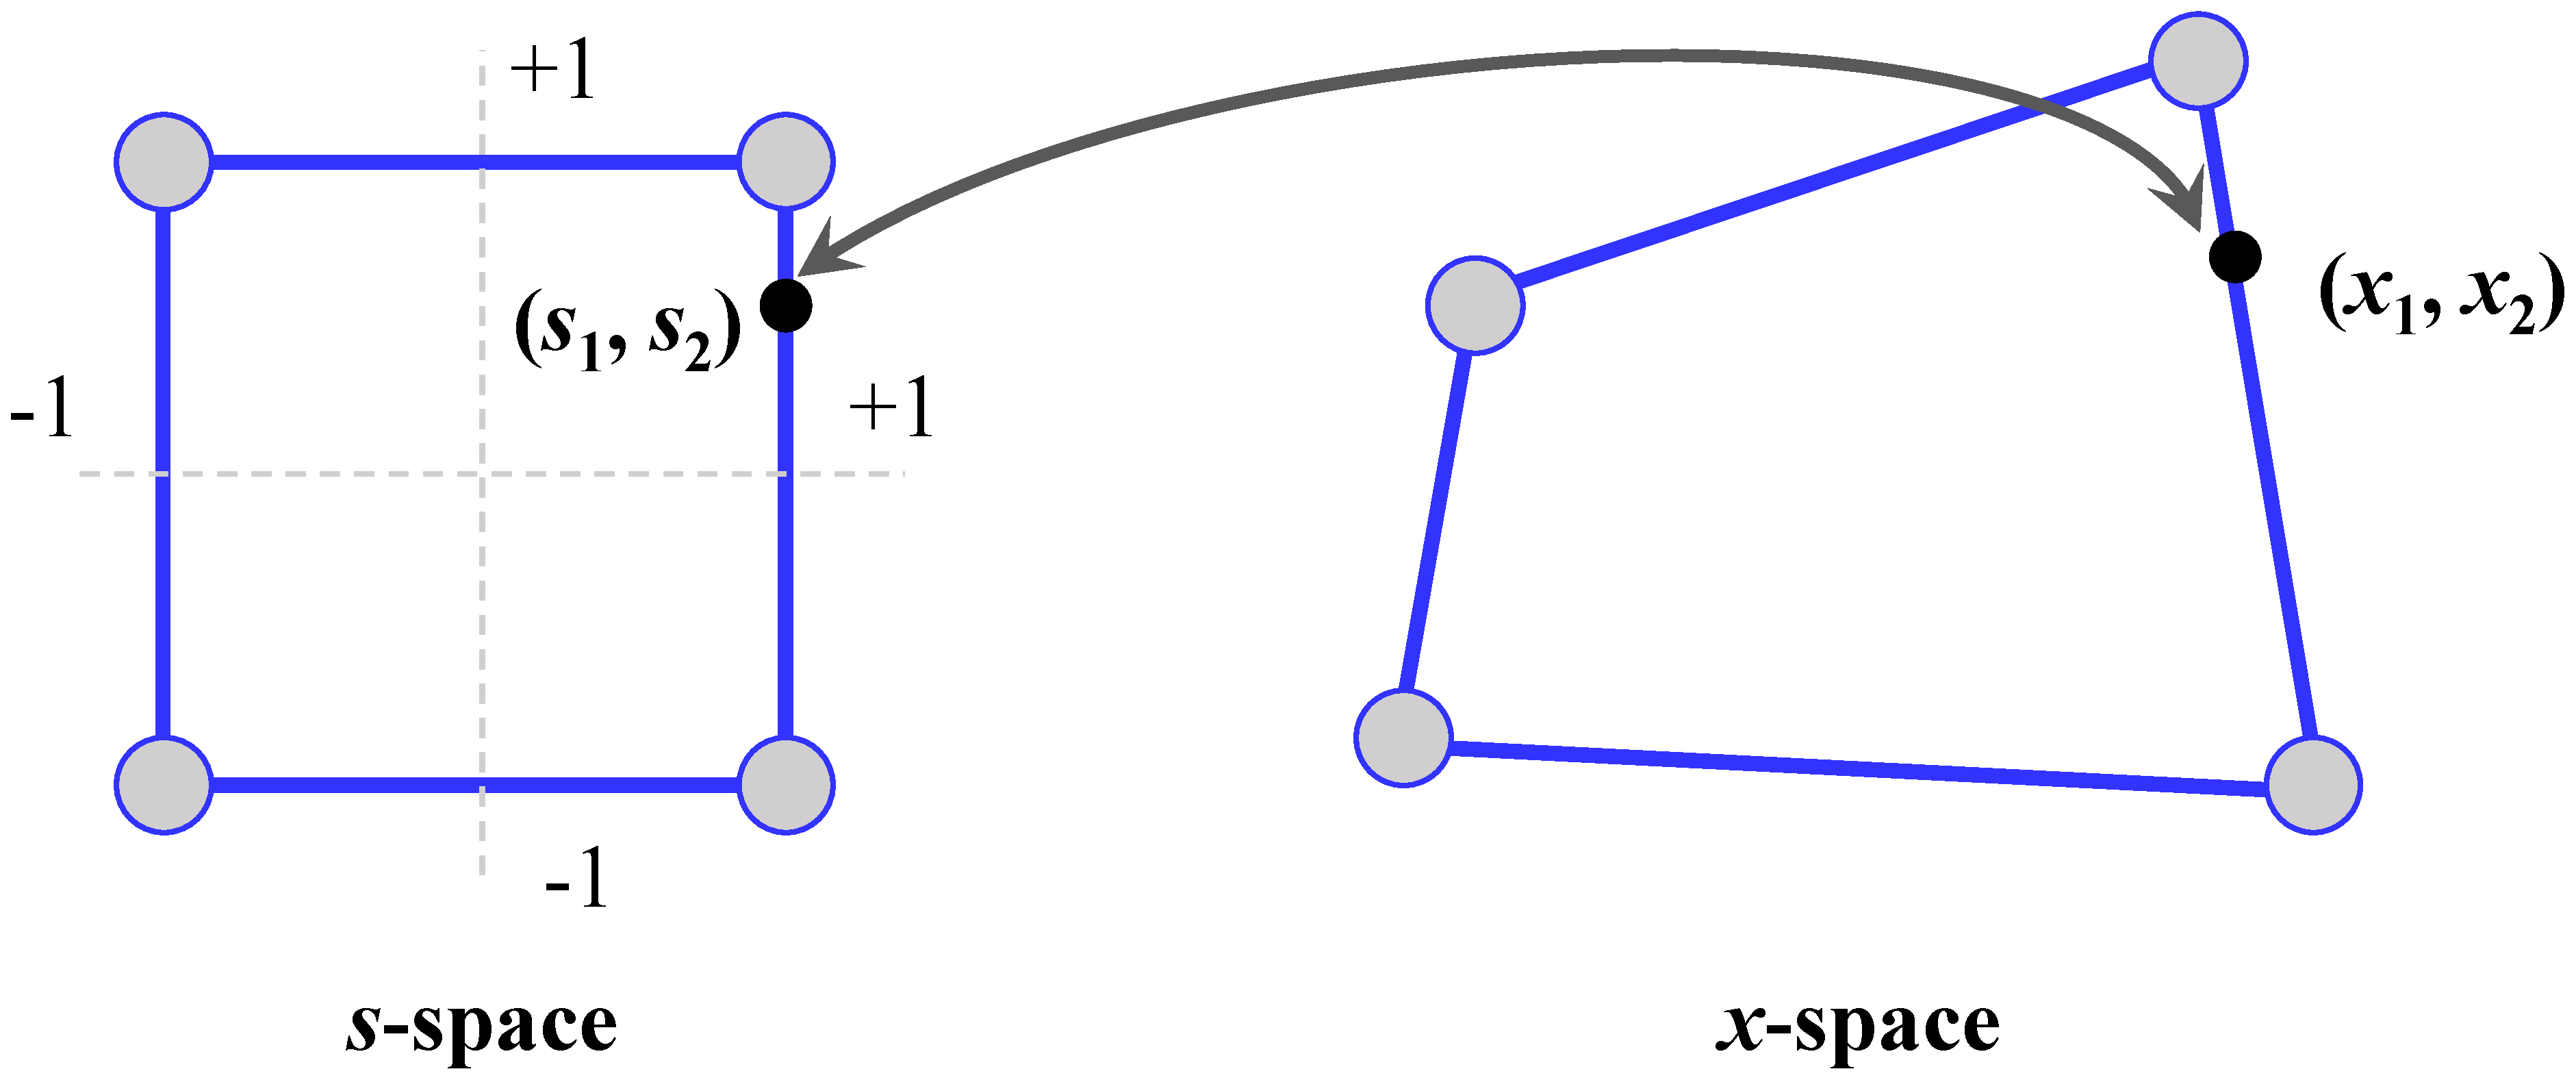
\includegraphics[width=0.7\linewidth]{figures/element_mapping.eps}
        \caption{Illustration of element mapping in FEA.}
        \label{fig:element_mapping}
    \end{figure}

In standard isoparametric finite elements, this mapping is constructed using the same \textit{shape functions} that are used to interpolate the displacement field. Therefore, before discussing Gaussian quadrature in detail, we first introduce the role of shape functions.

%==============================================================
\newpage
\subsection{Shape Function}
\label{sec:shape_function}

We start by looking at the shape functions in FEA. Shape functions are used to define the \textit{interpolate} deformation within the elements -- it can be deemed as the weights that blend nodal displacements.
\begin{equation}
\label{eqn:shape_function_interp}
    \mathbf{u}(\mathbf{x}) = \sum_{i=1}^{n} N_i(\mathbf{x})  \ \mathbf{u}_i.
\end{equation}
where $N_i$ is the shape function defined at node $i$, $n$ is the number of nodes of an element. 

\begin{remark}{}
    The interpolation of the deformation can be written in two equivalent forms: either in the shape function form (Equation~\ref{eqn:shape_function_interp}), or in the polynomial form. For example,
    \[
        u(x,y) = a_0 + a_1 x + a_2 y + a_3 x^2 + ...
    \]
\end{remark}

Shape functions depend on both the element's geometry and the interpolation function's order. Note that, an element shape function at node $a$, $N^e_a$, must obey the following rules:

\begin{enumerate}[label=(\alph*)]
    \item The value of a shape function at a node is either 0 or 1:
    $
    N_a^e =
    \begin{cases}
        1, & \text{at node $a$} \\
        0, & \text{otherwise}
    \end{cases}
    $ 
    
    \item The sum of all shape functions at any element node is equal to 1: $\displaystyle \sum_{a=1}^{NEL} N_a^e = 1$ where $NEL$ is the number of nodes per element.
    
    \item The value of shape functions are 0 ($N_a^e = 0$) outside element $e$.
\end{enumerate}

They are typically defined in the reference space: here we use $s_1$, $s_2$ to denote the axes in the parametric space.\\

In element mapping, shape functions of the parent elements are used in forming:
\begin{itemize}
    \item the mapping itself,
    \item the shape functions of the actual element,
    \item the derivatives,
    \item the change in areas (used in integral).
\end{itemize}

%% example
\begin{example}{Linear Shape Function of a Beam}
    Consider a 1-D beam element with 2 nodes. The nodes are designated to lie at $s = -1$ and $s = +1$ respectively. The lowest-order polynomial that can interpolate a function over the element is a linear function, as shown in Figure~\ref{fig:beam_lin_shape_fcn}.

    \begin{figure}[H]
        \centering
        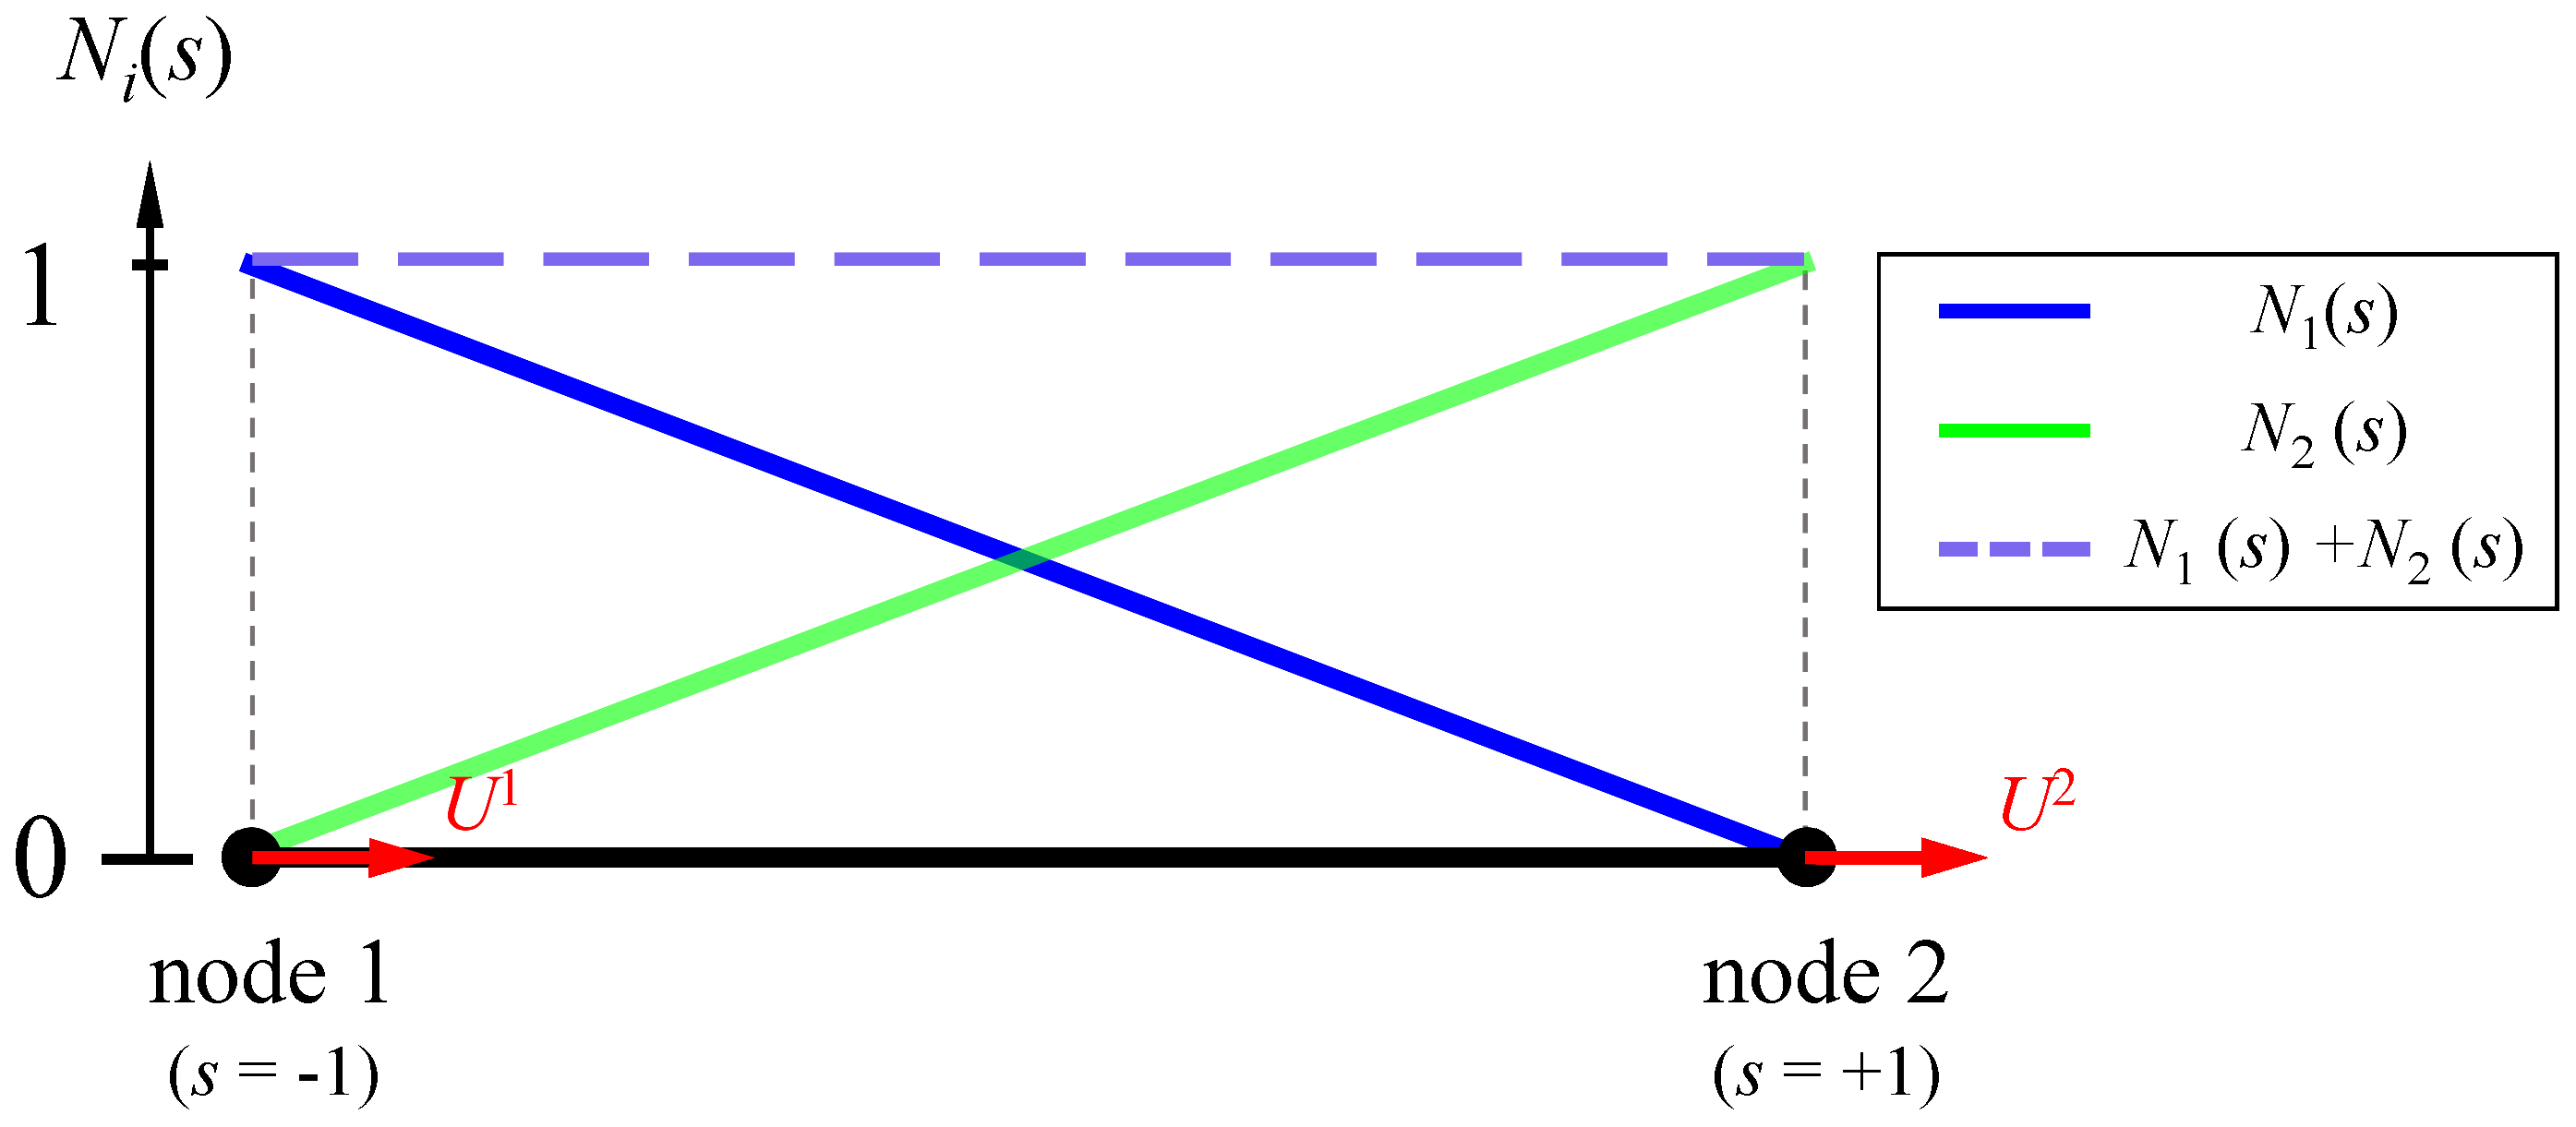
\includegraphics[width=0.7\linewidth]{figures/beam_lin_shape_fcn.eps}
        \caption{Linear shape functions $N_1$ and $N_2$ for a 2-node beam element.}
        \label{fig:beam_lin_shape_fcn}
    \end{figure}

    The shape functions for node 1 and 2 are denoted as $N_1$ and $N_2$, given by 
    \begin{equation*}
        N_1(s) = \frac{1}{2} (1-s), 
        \quad \quad
        N_2(s) = \frac{1}{2} (1+s).
    \end{equation*}

    Examine $N_1$ and $N_2$ to see whether they match the aforementioned rules for the shape functions:
    \begin{itemize}
        \item \textit{(Rule a)} At node 1 ($s=-1$), $N_1(-1) = 1$, $N_2(-1) = 0$ 
        \item \textit{(Rule a)} At node 2 ($s=+1$), $N_1(+1) = 0$, $N_2(+1) = 1$
        \item \textit{(Rule b)} At any point between $s=-1$ and $s=+1$, $N_1 + N_2 = 1$.
        \item \textit{(Rule c)} Outside the range $s\in[-1, 1]$, $N_1$ and $N_2$ are both 0, hence, $N_1 + N_2 = 0$.
    \end{itemize}
    
    Therefore, the interpolated displacement at any point between $s=-1$ and $s=+1$ is
    \begin{equation*}
        u(s) = \sum_{a=1}^{2} N_a (s) U^a = \frac{1}{2}(1-s)U^1 + \frac{1}{2}(1+s)U^2.
    \end{equation*}
    where $U_1$ and $U_2$ are the nodal displacement at node 1 and 2, respectively. For example, for $s=0$,
    \begin{equation*}
        u(0) = \frac{U^1 + U^2}{2}.
    \end{equation*}
    
\end{example}

% Example
\begin{example}{Quadratic Shape Function of a Beam}
    Similarly, quadratic interpolation over an element can also be used. The third node is usually lying halfway between the other two, providing more flexibility in describing the variation of $u$ within an element but also increasing the complexity of the problem.\\

    Consider the beam example, a third displacement node is added to the beam at $s=0$, and the corresponding shape functions $N_1$, $N_2$, $N_3$ are all quadratic:
    \begin{equation*}
        N_1(s) = \frac{s(s-1)}{2}, 
        \quad
        N_2(s) = \frac{s(s+1)}{2}, 
        \quad
        N_3(s) = 1 - s^2.
    \end{equation*}

    \begin{figure}[H]
        \centering
        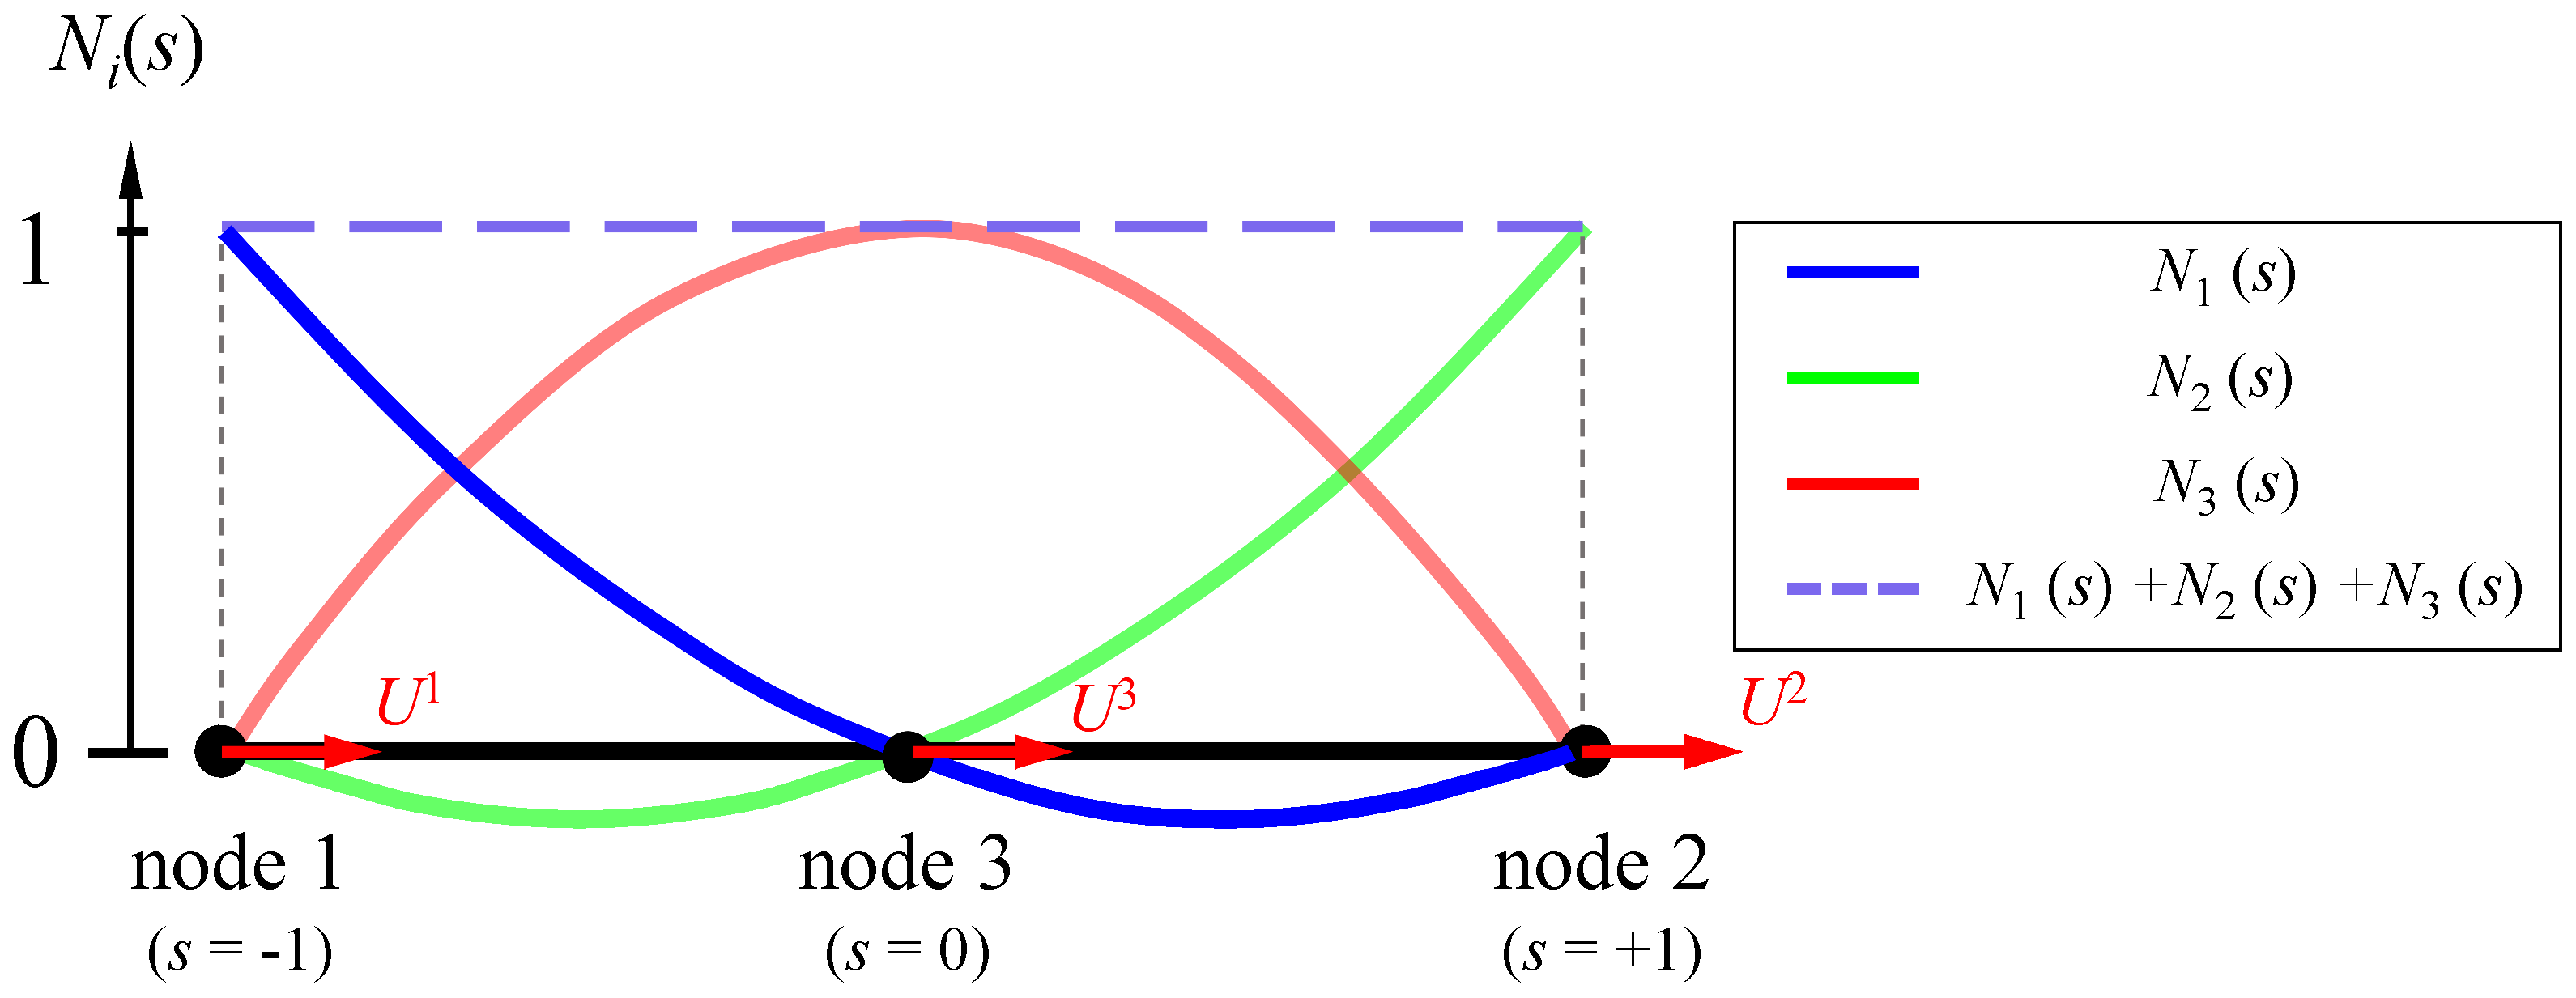
\includegraphics[width=0.8\linewidth]{figures/beam_quad_shape_fcn.eps}
        \caption{Quadratic shape functions $N_1$, $N_2$, and $N_3$ for a 3-node beam element.}
        \label{fig:beam_quad_shape_fcn}
    \end{figure}
\end{example}

For the more common two-dimensional elements, we can again describe them using bilinear or bi-quadratic elements. For example, the 2D bilinear shape functions for a quadrilateral element are
\begin{align}
\begin{split}
    N_1 (s_1, s_2) & = \frac{1}{4} (1-s_1) (1-s_2) \\
    N_2 (s_1, s_2) & = \frac{1}{4} (1+s_1) (1-s_2) \\
    N_3 (s_1, s_2) & = \frac{1}{4} (1+s_1) (1+s_2) \\
    N_4 (s_1, s_2) & = \frac{1}{4} (1-s_1) (1+s_2).
\end{split}
\end{align}
where the 4 nodes are labelled as shown in Figure~\ref{fig:quadrilateral}.

\begin{SCfigure}[1.5][!htbp]
    \centering
    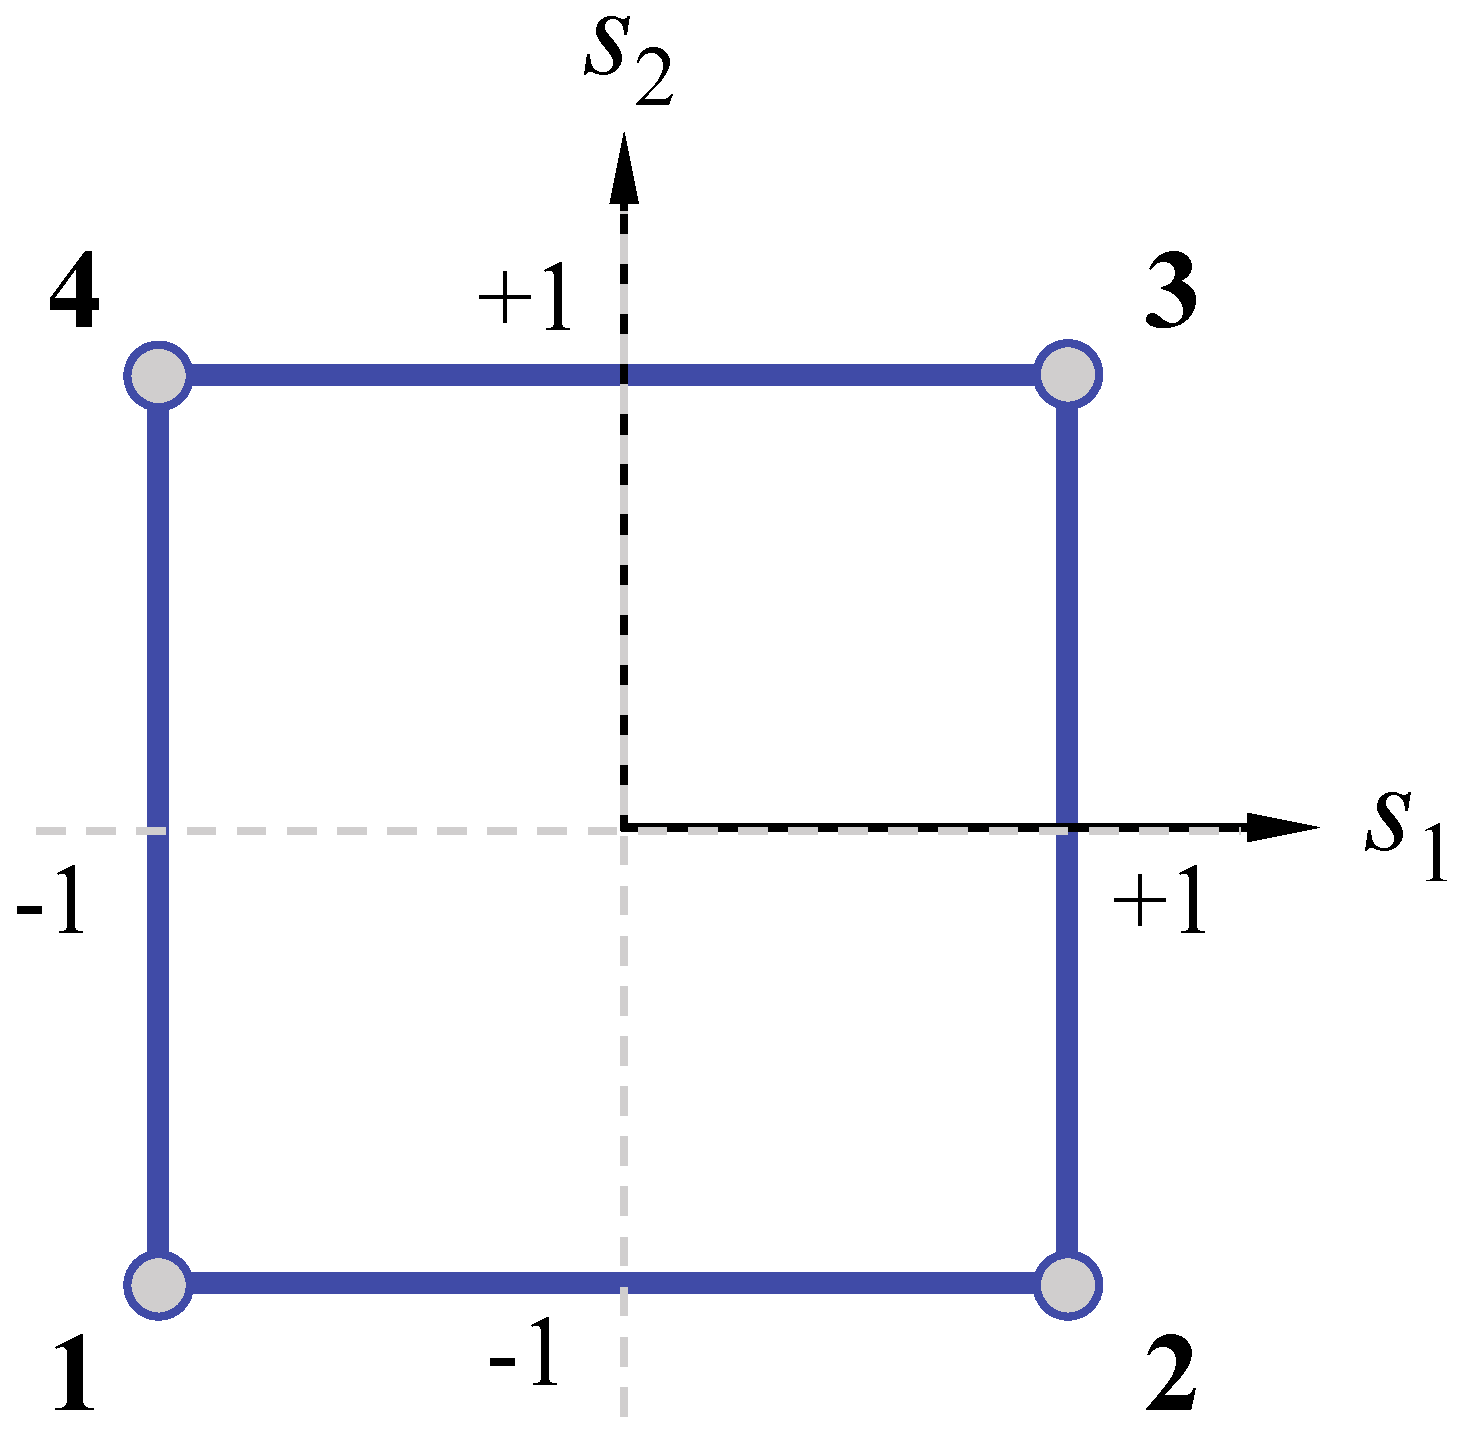
\includegraphics[width=0.3\linewidth]{figures/quadrilateral.eps}
    \caption{Four-node bilinear quadrilateral element in the parent $(s_1,s_2)$ reference space, with nodes numbered counterclockwise from the lower-left corner.}
    \label{fig:quadrilateral}
\end{SCfigure}

In standard FEM, the shape functions are chosen to be locally defined polynomials within each element, being zero outside the considered element,
\begin{equation*}
    N_a^{(e)}(\mathbf{x}) = 0, 
    \quad \text{if $\mathbf{x}$ not in element $(e)$},
\end{equation*}
and
\begin{equation*}
    \sum_{a=1}^{NEL} N_a^{(e)}(\mathbf{x}) = 1, \quad \text{for all $\mathbf{x} \in (e)$.}
\end{equation*}


\paragraph{Global shape function}
The global shape function, $N_a$, is assembled by stitching together local shape functions from neighbouring elements, $N_a^{(e)}$. See the explanations from the example below.

% Example
\begin{example}{Global Shape Function}
Consider a system comprised of three beam elements. For each 2-node beam element, it has node 1 (left) and node 2 (right); however, each element has its own \textit{local} numbering, while the full structure has a \textit{global} node numbering.
\begin{align*}
    \text{element 1}: \quad \text{local nodes 1, 2} \quad \leftrightarrow \quad \text{global nodes 1, 2} \\
    \text{element 2}: \quad \text{local nodes 1, 2} \quad \leftrightarrow \quad \text{global nodes 2, 3} \\
    \text{element 3}: \quad \text{local nodes 1, 2} \quad \leftrightarrow \quad \text{global nodes 3, 4} 
\end{align*}
Therefore, as illustrated in Figure~\ref{fig:global_n_local_nodes}, global node 2 corresponds to local node 2 in element 1 and local node 1 in element 2:
\[
\text{global node } 2
=
\text{local node } 2 \text{ of element } 1
=
\text{local node } 1 \text{ of element } 2.
\]
The shape function at global node 2 is therefore:
\[
    N_2(x)=
    \begin{cases}
    N_2^{(1)}(x), & x \in e^{(1)},\\
    N_1^{(2)}(x), & x \in e^{(2)},\\
    0, & \text{elsewhere}.
    \end{cases}
\]

\begin{figure}[H]
    \centering
    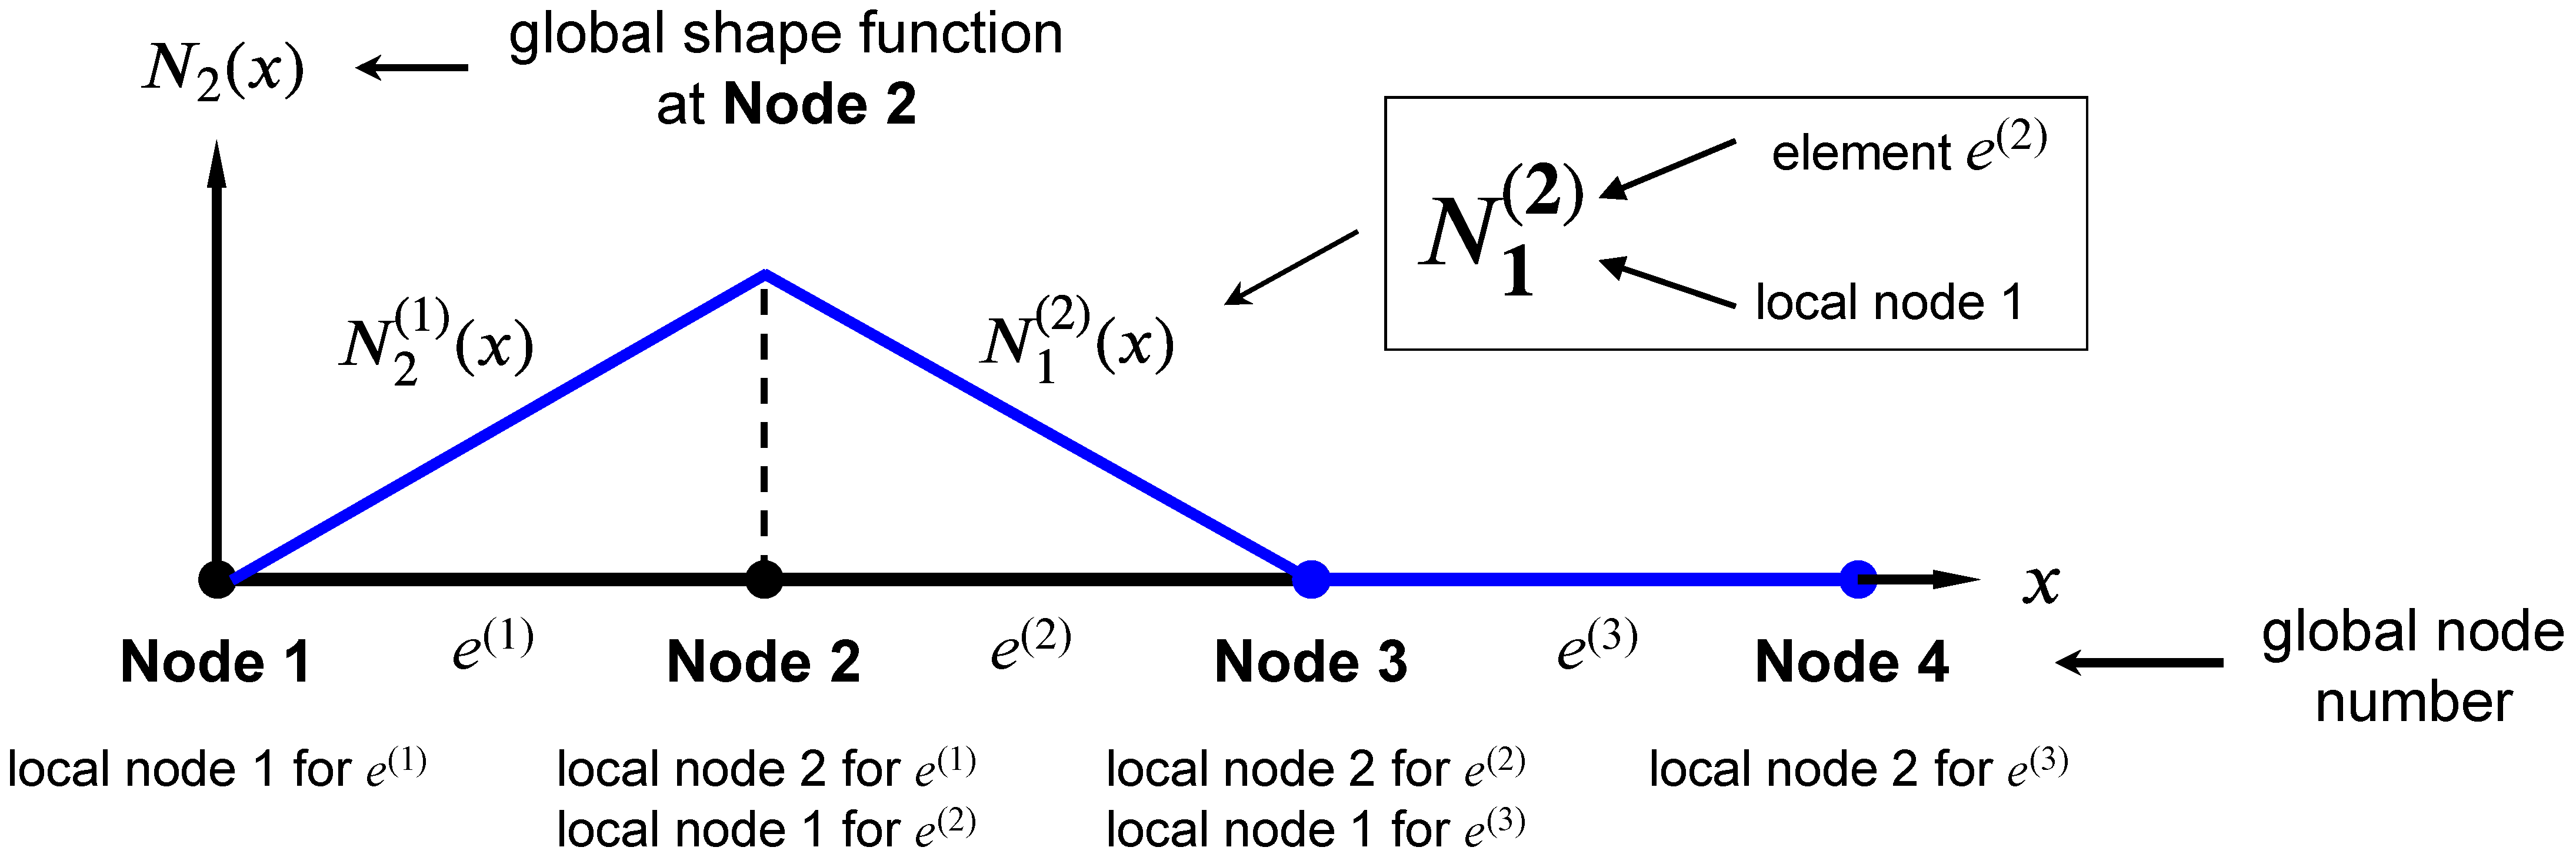
\includegraphics[width=\textwidth]{global_n_local_nodes.eps}
    \caption{Global shape function $N_2(x)$ of a 3-element 1-D element domain.}
    \label{fig:global_n_local_nodes}
\end{figure}
\end{example}

%==============================================================
\newpage
\subsection{Element Mapping}
\label{sec:element_mapping}

As shown in Section~\ref{sec:shape_function}, shape functions are used to interpolate the displacement field between the nodes within an element (Eq.~\eqref{eqn:shape_function_interp}). The same shape functions can be used to map the parent element to the physical element:

\begin{equation}
\label{eqn:isoparam_mapping}
    \mathbf{x}(\mathbf{s}) = \sum_{a=1}^{NEL} N_a(\mathbf{s}) \mathbf{x}_a
\end{equation}
where $\mathbf{s}$ denotes the coordinate vector in the reference space, $\mathbf{x}_a$ denotes the physical coordinates of node $a$, and $NEL$ is the number of nodes in the element.\\

Recall that this section aims to evaluate the element stiffness matrix -- how does the isoparametric mapping (Eq.~\eqref{eqn:isoparam_mapping}) assist the evaluation of $\kloc$? The key point is that the mapping transforms the integral in Eq.~\eqref{eqn:elem_stiff_matrix}, $\mathrm{d} V^e$, from the physical element domain to the standard parent element domain:
\begin{align}
    \begin{split}
        \mathrm{d} V^e 
        & = \mathrm{d}x_1 \mathrm{d} x_2 \\
        & = \det([\mathbf{J}]) \ \mathrm{d} s_1 \mathrm{d} s_2.
    \end{split}
\end{align}
where $[\mathbf{J}] = \dfrac{\partial \mathbf{x}}{\partial \mathbf{s}}$ is the Jacobian matrix of $\mathbf{x}$, satisfying 
\begin{equation}
    \begin{bmatrix}
        \delta x_1 \\
        \delta x_2 
    \end{bmatrix}
    = 
    \underbrace{\begin{bmatrix}
    \dfrac{\partial x_1}{\partial s_1} &
    \dfrac{\partial x_1}{\partial s_2} \\[2.5ex]
    \dfrac{\partial x_2}{\partial s_1} &
    \dfrac{\partial x_2}{\partial s_2} \\
    \end{bmatrix}}_{[\mathbf{J}]}
    \begin{bmatrix}
        \delta s_1 \\
        \delta s_2 
    \end{bmatrix}.
\end{equation}

Now, revisiting Eq.~\eqref{eqn:elem_stiff_matrix}:
\begin{align}
    \kloc 
    & = \int\limits_{\Omega^{e}} \B^\top \D \B \ \mathrm{d} V^e \nonumber \\
    & = \iint \B^\top \D \B \mathrm{d}x_1 \mathrm{d}x_2 \nonumber \\
    & = \boxed{\int_{-1}^{+1} \int_{-1}^{+1} \B^\top \D \B \det([\mathbf{J}]) \ \mathrm{d} s_1 \mathrm{d} s_2.} \label{eqn:kloc_map}
\end{align}

Note that the upper and lower boundaries of Eq.~\eqref{eqn:kloc_map} are now mapped into the standard interval $[-1, 1]$ in the reference domain -- this is a deliberate choice, as selecting the integration limits as $-1$ and $1$ allows the Gaussian quadrature to be applied conveniently.

%==============================================================
\newpage
\subsection{Gaussian Quadrature}
\label{section:num_quadrature}

The core idea of the Gaussian quadrature is to approximate a definite integral (which spans the domain $[-1, 1]$) as the weighted sum of function values evaluated at selected points, as detailed later in Eq.~\eqref{eqn:O1_quadrature}. \\

It is worth noting that these selected points -- often called \textit{Gauss points} -- are chosen optimally (rather than sampled uniformly or arbitrarily), so that a Gaussian quadrature formula using $n$ points can exactly integrate polynomials of degree up to $2n−1$.

\paragraph{One-Dimensional Gaussian Quadrature}
The one-dimensional integral can be replaced by a sum
\begin{equation}
\label{eqn:O1_quadrature}
    I = \int_{-1}^{+1} f(s) \ \mathrm{d}s \ \approx \ \sum_{p=1}^{NQP} w_p f(\xi_p),
\end{equation}
where $NQP$ denotes the number of quadrature (Gauss) points; $\xi_p$ give the position of Gauss points, and $w_p$ are the weights applied to each Gauss points. 

\begin{table}[h!]
    \centering
    \begin{tabular}{ccc}
    \toprule
        $NQP$   &   $\xi$   &   $w$ \\
    \toprule
        1 &  0  &   2\\
    \midrule
        2 & $-\frac{1}{\sqrt{3}}$ and $+\frac{1}{\sqrt{3}}$ &   1 and 1 \\
    \midrule
        3 &  $-\sqrt{\frac{3}{5}}$ and 0 and $+\sqrt{\frac{3}{5}}$ &   $\frac{5}{9}$ and $\frac{8}{9}$ and $\frac{5}{9}$ \\
    \midrule
        4 & $-\sqrt{\frac{3}{7}+\frac{2}{7}\sqrt{\frac{6}{5}}}$   &   $\frac{18-\sqrt{30}}{36}$ \\
        & $+\sqrt{\frac{3}{7}+\frac{2}{7}\sqrt{\frac{6}{5}}}$   &   $\frac{18-\sqrt{30}}{36}$ \\
        & $-\sqrt{\frac{3}{7}-\frac{2}{7}\sqrt{\frac{6}{5}}}$   &   $\frac{18+\sqrt{30}}{36}$ \\
        & $+\sqrt{\frac{3}{7}-\frac{2}{7}\sqrt{\frac{6}{5}}}$   &  $\frac{18+\sqrt{30}}{36}$ \\
    \bottomrule
    \end{tabular}
    \caption{Location of Gauss points and magnitudes of weights for $NQP$ = 1 to 4}
    \label{tab:quadrature}
\end{table}

\begin{example}{Derivation of the One-Point Gauss Rule}
Consider the following integration problems using one Gauss point ($NQP = 1$):

\begin{itemize}
    \item For a constant function  $f(s) = 1$, \begin{align*}
        \int_{-1}^{1} 1 \ \mathrm{d}s = 2 \ ,
        \quad \quad
        & \sum_{p=1}^{1} w_p f(\xi_p) = w_1 \times 1 = w_1 \\
        & \Rightarrow w_1 = 2 \ .
    \end{align*}

    \item Next, for a linear function $f(s) = s$,
    \begin{align*}
        \int_{-1}^{1} s \ \mathrm{d}s = 0 \ ,
        \quad \quad
        & \sum_{p=1}^{1} w_p f(\xi_p) = w_1 \times \xi_1 = 2 \xi_1 \\
        & \Rightarrow \xi_1 = 0 \ .
    \end{align*}
\end{itemize} 

Therefore, the one-point Gauss rule on the interval $[-1,1]$ is given by
\begin{equation}
\label{eqn:NQP1_quadrature}
    \int_{-1}^{1} f(s) \ \mathrm{d}s \approx 2 f(0). \tag{\star}
\end{equation}
That is, for $NQP=1$, the Gauss point is located at $\xi=0$ (taking the midpoint of the interval [-1, 1]), and the corresponding weight is $w=2$, which matches the first row in Table~\ref{tab:quadrature}. \\

Also, you may realise that, for any linear function of the form $f(s)=a_0+a_1s$, the expression of Eq.~\eqref{eqn:NQP1_quadrature} is exact:
\begin{align*}
    \int_{-1}^{1} (a_0+a_1s) \ \mathrm{d}s
    &= 2a_0, \\
    2f(0)
    &= 2(a_0+a_1 \cdot 0)
    = 2a_0.
\end{align*}
Hence, one-point Gaussian quadrature is exact for polynomial functions of degree up to 1, which is consistent with the general result that an $n$-point Gauss rule is exact up to degree $2n-1$.
\end{example}


\paragraph{Two-Dimensional Gaussian Quadrature}
\begin{align}
\label{eqn:quadrature}
    \int_{-1}^{+1} \int_{-1}^{+1} f(s_1, s_2) \ \mathrm{d}s_1 \ \mathrm{d} s_2 
    & = \int_{-1}^{+1} \left[ \sum_{p=1}^{NQP} w_p f(\xi_p, s_2) \right] \mathrm{d} s_2 \nonumber \\
    & = \sum_{p=1}^{NQP} w_p \left[ \int_{-1}^{+1} f(\xi_p, s_2) \mathrm{d} s_2  \right] \nonumber \\
    & = \sum_{p=1}^{NQP} w_p \left[ \sum_{q=1}^{NQP} w_q f(\xi_p, \xi_q) \right] \nonumber \\
    & = \sum_{p=1}^{NQP} \sum_{q=1}^{NQP} w_p w_q f(\xi_p, \xi_q) .
\end{align}

\begin{SCfigure}[1][!htbp]
    \centering
    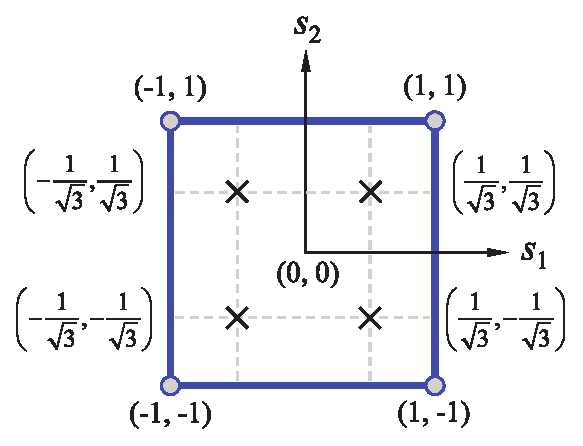
\includegraphics[width=0.45\linewidth]{figures/quadrature.eps}
    \caption{Locations of the Gauss points $(\xi_p,\xi_q)$ for a $2\times2$ Gaussian quadrature rule on the parent element in the $(s_1,s_2)$ reference space.}
    \label{fig:quadrature}
\end{SCfigure}

%==============================================================
\newpage
\subsection{Evaluating the Element Stiffness Matrix Using Quadrature}

In Section~\ref{sec:element_mapping}, we have derived the element stiffness matrix after isoparametric mapping (Eq.~\eqref{eqn:kloc_map})
\[
    \kloc = \int_{-1}^{+1} \int_{-1}^{+1} \B^\top \D \B \det([\mathbf{J}]) \ \mathrm{d} s_1 \mathrm{d} s_2.
\]
This expression can be finally evaluated by applying the numerical quadrature following Eq.~\eqref{eqn:quadrature}:
\begin{equation}
    \kloc = \sum_{p=1}^{NQP} \sum_{q=1}^{NQP} w_p w_q \B^\top (\xi_p, \xi_q) \D \B (\xi_p, \xi_q) \det([\mathbf{J}]) (\xi_p, \xi_q) \ ,
\end{equation}
which is the final expression of the local stiffness matrix. \\

One can further find $\B$, which is the derivative of the shape function w.r.t. to the \textit{physical} space coordinates, 
\begin{equation}
    \B = \frac{\partial N_a}{\partial x_j} = \frac{\partial N_a}{\partial s_i} \left( \frac{\partial s_i}{\partial x_j} \right)
    = \left( \frac{\partial N_a}{\partial s_i} \right) [\mathbf{J}]^{-1} .
\end{equation}
Mind that, since shape functions are usually defined in the \textit{reference} space, the chain rule is employed to find the derivatives. This process involves calculating the determinant of the Jacobian, as 
\begin{equation*}
    \det([\mathbf{J}])  = \det \left( \frac{\partial x_i}{\partial s_j} \right) =  \frac{\partial x_1}{\partial s_1} \frac{\partial x_2}{\partial s_2} - \frac{\partial x_1}{\partial s_2} \frac{\partial x_2}{\partial s_1} .
\end{equation*}


%==============================================================
\newpage
\section{Principle of Virtual Work}
%==============================================================

We shall now derive the equation
\[
    \kloc = \int\limits_{\Omega^{e}} \B^\top \D \B \ \mathrm{d} V^e.
\]
The following derivation is based on the \textit{principle of virtual work} (PVW). Rigorously, PVW is not equivalent to the variational form:
\begin{itemize}
    \item PVW is a physics-based principle from a perspective of energy equilibrium, whereas the variational form is the mathematical minimisation of the functional. 

    \item However, they are closely related, and share very similar procedures when applying to the problem, hence not surprisingly yielding the same solution. 
\end{itemize}

\paragraph{Problem Definition}
Consider a static structural problem as shown in Figure \ref{fig:virtual_work}, the body is defined in the domain $\Omega$, with the boundary $\Gamma = \Gamma_t \cup \Gamma_u$. The displacement $u_i^s$ is specified on the boundary $\Gamma_u$, whereas the surface traction $f^s_i$, is defined on the boundary $\Gamma_t$. 
\begin{figure}[ht!]
    \centering
    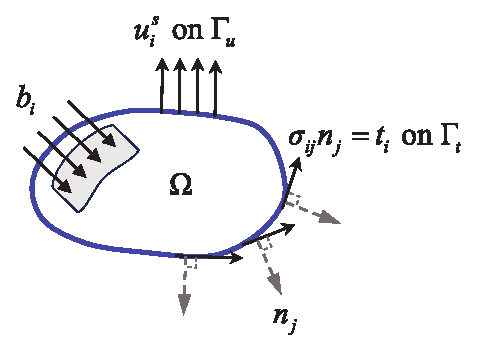
\includegraphics[width=0.5\linewidth]{virtual_work.eps}
    \caption{A mechanical body $\Omega$ subject to displacements and tractions.}
    \label{fig:virtual_work}
\end{figure}

This allows us to formulate the governing equations as
\begin{align}
    \text{(Equilibrium)} \quad \quad & \rho \ddot{u}_i - \sigma_{ij, j} - \rho b_i = 0, & \text{in $\Omega$} \\
    \text{(Displacement BC)} \quad \quad & u_i = u_i^s , & \text{on $\Gamma_u$} \\
    \text{(Traction BC)} \quad \quad & \sigma_{ij} n_j = t_i & \text{on $\Gamma_t$}
\end{align}
where $\sigma_{ij, j}$ represents the internal stresses, $\rho b_i$ represents the external forces, and $\rho \ddot{u}_i$ is the inertial effects. \\ 

The \textit{aim} is seeking the displacement field, $u$, that satisfies all equations listed above.

\paragraph{Principle of Virtual Work} 
For a solid body undergoing small deformation, we introduce a virtual displacement field, $\delta u_i$, which is bounded within the domain $\Omega$. Note that there is no displacement on the displacement boundary, \textit{i.e.}, $\delta u_i = 0$ on $\Gamma_u$. The principle of virtual work states that 
\begin{equation}
\label{eqn:vit_work1}
    \int \limits_\Omega \delta u_i \cdot (\rho \ddot{u}_i - \rho b_i) \ \mathrm{d}V - 
    \int \limits_\Omega \delta u_i \cdot \sigma_{ij, j} \  \mathrm{d}V
    + \int \limits_{\Gamma_t} \delta u_i \cdot(\sigma_{ij} n_j - t_i) \mathrm{d}A = 0.
\end{equation}
For further simplifications of Equation~\ref{eqn:vit_work1}, the second term $\delta u_i \cdot \sigma_{ij, j}$ can be decomposed into the combination of $(\delta u_i \sigma_{ij})_{,j}$ and $\sigma_{ij} \cdot \delta u_{i,j}$:
\begin{align}
\begin{split}
\label{eqn:vit_work2}
    \int \limits_\Omega  \delta u_i \cdot \sigma_{ij, j} \ \mathrm{d}V
    & = \int \limits_\Omega \frac{\partial}{\partial x_j} \sigma_{ij} \cdot \delta u_i \ \mathrm{d}V \\
    & = \int \limits_\Omega \frac{\partial}{\partial x_j} (\sigma_{ij} \delta u_i) \ \mathrm{d}V - \int \limits_\Omega \sigma_{ij} \bigg(\frac{\partial}{\partial x_j} \delta u_i \bigg) \ \mathrm{d}V.
\end{split}
\end{align}
Next, applying the divergence theorem to the first term on the R.H.S. of Equation~\ref{eqn:vit_work2}, the volume integral can be converted into the surface integral,
\begin{equation}
\label{eqn:vit_work3}
    \int \limits_\Omega \frac{\partial}{\partial x_j} (\sigma_{ij} \delta u_i)_{, j} \ \mathrm{d}V = \int \limits_\Gamma \sigma_{ij} \delta u_i n_j \ \mathrm{d}A , 
\end{equation}
where $\mathbf{n}$ is the unit normal vector to the surface $\Gamma$. Since $\Gamma \equiv \Gamma_u \cup \Gamma_t$, and recall that $\delta u_i = 0$ on $\Gamma_u$,
\begin{equation}
\label{eqn:vit_work4}
    \int \limits_\Gamma \sigma_{ij} \delta u_i n_j \ \mathrm{d} A
    = \int \limits_{\Gamma_u + \Gamma_t} \sigma_{ij} \delta u_i n_j \ \mathrm{d} A \\
    = \int \limits_{\Gamma_t} \sigma_{ij} \delta u_i n_j \ \mathrm{d} A.
\end{equation}
Substituting Equation~\ref{eqn:vit_work4} back to Equation~\ref{eqn:vit_work2},
\begin{align}
\begin{split}
\label{eqn:vit_work5}
    \int \limits_\Omega \sigma_{ij, j} \delta u_i \ \mathrm{d}V
    & = \int \limits_{\Gamma_t} \sigma_{ij} \delta u_i n_j \ \mathrm{d}A - \int \limits_\Omega \sigma_{ij} \bigg(\frac{\partial}{\partial x_j} \delta u_i \bigg) \ \mathrm{d}V \\
    & = \int \limits_{\Gamma_t} \sigma_{ij} \delta u_i n_j \ \mathrm{d}A - \int \limits_\Omega \sigma_{ij} \delta u_{i,j} \ \mathrm{d}V .
\end{split}
\end{align}
By mapping Equation~\ref{eqn:vit_work5} back to Equation \ref{eqn:vit_work1}, the overall balance of force
\begin{equation}
\label{eqn:vit_weak}
    \int \limits_\Omega \delta u_i \cdot \rho \ddot{u}_i \ \mathrm{d}V 
    + \int \limits_\Omega \sigma_{ij} \ \delta u_{i, j} \  \mathrm{d}V
    \cancel{- \int \limits_{\Gamma_t} \delta u_i \cdot \sigma_{ij} n_j \ \mathrm{d}A}
    = 
    \int \limits_\Omega \delta u_{i} \cdot \rho b_i\  \mathrm{d}V
    - \int \limits_{\Gamma_t} \delta u_i (\cancel{\sigma_{ij} n_j} - t_i) \ \mathrm{d}A,
\end{equation}
which is known as the \textit{weak} form of the momentum balance equation (or, the principle of virtual work). The term $\delta u$ is the virtual displacement field. \\

Next, we shall separate the summands in Equation~\ref{eqn:vit_weak} into the virtual work terms:
\begin{align}
    \delta W_{\rm dyn} &= \int \limits_\Omega \delta u_i \cdot \rho \ddot{u}_i \ \mathrm{d}V \\
    \delta W_{\rm int} &= \int \limits_\Omega \sigma_{ij} \ \delta u_{i, j} \  \mathrm{d}V \\
    \delta W_{\rm ext} &= \int \limits_\Omega \delta u_{i} \cdot \rho b_i\  \mathrm{d}V + \int \limits_{\Gamma_t} \delta u_i \cdot t_i \ \mathrm{d}A,
\end{align}
where $\delta W_{i}$, $i \in \{\mathrm{dyn}, \mathrm{int}, \mathrm{ext}\}$ denote the virtual work of inertial forces, internal forces, and external forces, respectively, satisfying:
\begin{equation}
    \delta W_{\rm dyn} + \delta W_{\rm int} = \delta W_{\rm ext}.
\end{equation}

For the virtual work done by internal force, one further simplification is that the term $\sigma_{ij} \delta u_{i,j}$ can be written as $\sigma_{ij} \delta \varepsilon_i$, which can be proved by
\begin{equation}
    \frac{1}{2} (\delta u_{i,j} + \delta u_{j,i}) \sigma_{ij} = \frac{1}{2} (\delta u_{i,j} \sigma_{ij} + \delta u_{j,i} \sigma_{ij}) = \frac{1}{2} (\delta u_{i,j} \sigma_{ij} + \delta u_{i,j} \sigma_{ij}) = \delta u_{i,j} \sigma_{ij}.
\end{equation}
Now, by $\stress = \D \strain$, and $\strain = \B \bu$,
\begin{equation}
\label{eqn:int_energy_weak}
    \delta W_{\rm int} 
    = \int \delta \boldsymbol{\varepsilon} : \stress \ \mathrm{d}V
    = \int \limits_\Omega \B^\top \D \B \bu \delta u \ \mathrm{d}V, 
\end{equation}

Now, if we neglect the existence of $\delta W_{\rm dyn}$, and the virtual work done by external forces is 
\begin{equation}
    \delta W_{\rm ext} = \int \limits_\Omega \delta u_{i} \cdot \rho b_i\  \mathrm{d}V
\end{equation}
We can therefore write the weak form of the momentum balance equation as
\begin{equation}
    \int \limits_\Omega \B^\top \D \B \bu \delta u \ \mathrm{d}V = \int \limits_\Omega \delta u_{i} \cdot \rho b_i\  \mathrm{d}V 
    \quad \Rightarrow \quad
    \int \limits_\Omega \B^\top \D \B \bu - \rho \mathbf{b} \ \mathrm{d}V = 0
\end{equation}
The fundamental lemma of variation calculus states that for an arbitrary choice of $\delta u$, the integrated expression must be 0:
\[
    \int \limits_\Omega (\star) \ \delta u \ \mathrm{d}V  \quad \Rightarrow \quad (\star) = 0.
\]
Hence, we may state 
\begin{equation}
     \underbrace{\B^\top \D \B}_{\kloc} \bu - \mathbf{b} = 0 \quad \Rightarrow \quad
     \kloc \bu =  \mathbf{b}
\end{equation}
where $\kloc$ is the element (local) stiffness matrix. This final expression matches the strong form of the equation we have seen previously.

%==============================================================
\newpage
\section{Continuum Mechanics and Nonlinear FEM}
%==============================================================
\subsection{Kinematics: Deformation and Strain Measures}

\subsubsection{The Deformation Gradient Tensor, $\bF$}

Consider the deformation of a continuum as depicted by Figure~\ref{fig:configs}, the initial domain $\Omega_0$ is deformed to the current domain $\Omega_x$.\\

\begin{figure}[ht!]
    \centering
    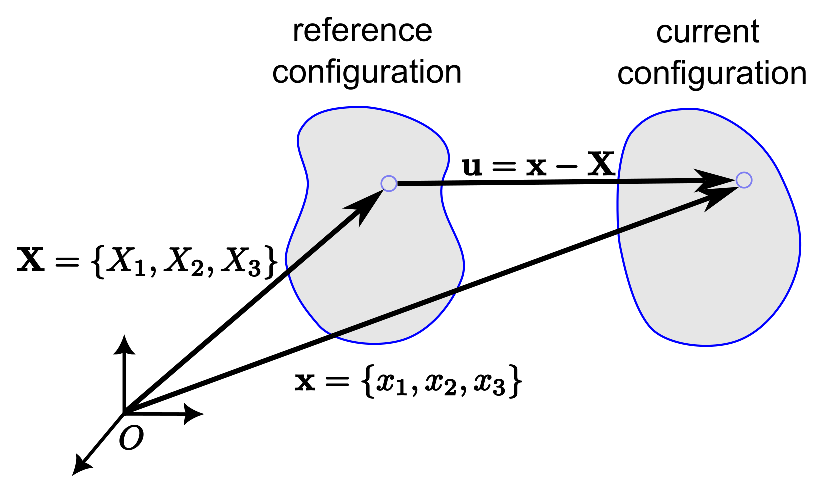
\includegraphics[width=0.6\linewidth]{ref_configuration.eps}
    \caption{Reference configuration and deformed configuration}
    \label{fig:configs}
\end{figure}

In Figure~\ref{fig:configs}, ${\bf X} \equiv \{X_1, X_2, X_3\} \in \Omega_0$ is a material point in the \textit{reference (initial) configuration}, and ${\bf x} \equiv \{x_1, x_2, x_3\} \in \Omega_x$ is a material point in the \textit{deformed (current) configuration}. This deformation process can be thought of as a mapping from $\Omega_0$ to $\Omega_x$. \\

If the deformation vector (displacement) is given by $\bf u$, and the mapping operator is given by $\chi$, 
\begin{equation}
    {\bf x} = \chi({\bf X}, t) = {\bf X} + {\bf u}({\bf X}, t)
\end{equation}
Hence, the deformation vector 
\begin{equation}
    {\bf u}({\bf X}, t) = {\bf x}({\bf X}, t) - {\bf X},
\end{equation}
which is known as the Lagrangian (material) description of motion. Now, consider an infinitesimal length, $\mathrm{d} {\bf X} \in \Omega_0$ that deforms to $\mathrm{d} {\bf x} \in \Omega_x$, 
\begin{equation}
    \mathrm{d} {\bf x} = \frac{\mathrm{d} {\bf x}}{\mathrm{d} {\bf X}} \cdot \mathrm{d} {\bf X}
\end{equation}
where the term $\dfrac{\mathrm{d} {\bf x}}{\mathrm{d} {\bf X}}$ is known as the \textit{deformation gradient tensor} $\bF$, 
\begin{equation}
    \bF = \frac{\mathrm{d} {\bf x}}{\mathrm{d} {\bf X}} = 
    \begin{bmatrix}
        \dfrac{\partial x_1}{\partial X_1} & \dfrac{\partial x_1}{\partial X_2} & \dfrac{\partial x_1}{\partial X_3} \\[3ex]
        \dfrac{\partial x_2}{\partial X_1} & \dfrac{\partial x_2}{\partial X_2} & \dfrac{\partial x_2}{\partial X_3} \\[3ex]
        \dfrac{\partial x_3}{\partial X_1} & \dfrac{\partial x_3}{\partial X_2} & \dfrac{\partial x_3}{\partial X_3} \\
    \end{bmatrix}
\end{equation}

The deformation gradient tensor, $\bF$, can be expressed as
\begin{equation}
\label{eqn:deform_grad}
    \bF 
    = \frac{\mathrm{d} {\bf x}}{\mathrm{d} {\bf X}} 
    = \frac{\mathrm{d}}{\mathrm{d} {\bf X}} (\mathbf{u} + \mathbf{X}) 
    = \frac{\mathrm{d} {\bf u}}{\mathrm{d} {\bf X}} + \underbrace{\frac{\mathrm{d} {\bf X}}{\mathrm{d} {\bf X}}}_{= \II} 
    \ \boxed{= \frac{\mathrm{d} {\bf u}}{\mathrm{d} {\bf X}} + \II}.
\end{equation}

The determinant of $\bF$ is known as the Jacobian of deformation, $J$,
\begin{equation}
    J = \det (\bF).
\end{equation}
Due to one-to-one mapping, $J>0$, and the inverse mapping exists as 
\begin{equation}
    \mathrm{d}{\bf X} = \bF^{-1} \mathrm{d}{\bf x}.
\end{equation}

\paragraph{Remark} The deformation gradient, $\bf F$, describes how a line element in the reference configuration maps into a line element in the current configuration. It gives information about deformation and rigid body rotation, but not rigid body translations. 

%==============================================================
\subsubsection{Cauchy--Green Deformation Tensors}
\paragraph{Right Cauchy--Green Deformation Tensor, $\bf C$} Consider two line elements in the reference configuration, $\mathrm{d} {\bf X}^{(1)}$ and $\mathrm{d} {\bf X}^{(2)}$ which are mapped into the line elements $\mathrm{d} {\bf x}^{(1)}$ and $\mathrm{d} {\bf x}^{(2)}$ in the current configuration, respectively. The mapping can be expressed as
\begin{align}
    \mathrm{d} {\bf x}^{(1)} \cdot \mathrm{d} {\bf x}^{(2)}
    & = (\bF \mathrm{d} {\bf X}^{(1)}) \cdot (\bF \mathrm{d} {\bf X}^{(2)}) \nonumber \\[.5em]
    & = \mathrm{d} {\bf X}^{(1)} \ (\bF^{\top} \bF) \ \mathrm{d} {\bf X}^{(2)} \nonumber \\[.5em]
    & = \mathrm{d} {\bf X}^{(1)} \ \bC \ \mathrm{d} {\bf X}^{(2)}
\end{align}
where, by definition, $\bC$ is the right Cauchy--Green deformation tensor. By means of ``right'', the deformation gradient $\bf F$ is on the right of the formula:
\begin{equation}
    \bC = \bF^\top  \bF \quad \text{or} \quad
    C_{ij} = F_{ki} F_{kj}
\end{equation}
As seen, $\bC$ is defined in and associated with the reference configuration, acting on vectors in the reference configuration; therefore, it is also called a \textbf{material tensor}.

\paragraph{Left Cauchy--Green Deformation Tensor, $\bf b$} Now, consider the line elements defined in the current configuration and maps back to the reference configuration:
\begin{align}
    \mathrm{d} {\bf X}^{(1)} \cdot \mathrm{d} {\bf X}^{(2)}
    & = (\bF^{-1} \mathrm{d} {\bf x}^{(1)}) \cdot (\bF^{-1} \mathrm{d} {\bf x}^{(2)}) \nonumber \\[.5em]
    & = \mathrm{d} {\bf x}^{(1)} \ (\bF^{-\top} \bF^{-1}) \ \mathrm{d} {\bf x}^{(2)} \nonumber \\[.5em]
    & = \mathrm{d} {\bf x}^{(1)} \ \bb^{-1} \ \mathrm{d} {\bf x}^{(2)}
\end{align}
where, by definition, $\bf b$ is the left Cauchy--Green deformation tensor:
\begin{equation}
    \bb = \bF  \bF^\top \quad \text{or} \quad
    b_{ij} = F_{ik} F_{jk}.
\end{equation}
As $\bf b$ is defined in and associated with the current configuration, it is also called a spatial tensor.

---

\paragraph{Remark a.} Both $\bf C$ and $\bf b$ are symmetric, such that
\[
    \bC^\top 
    = (\bF^\top \bF)^\top 
    = \bF^\top (\bF^\top)^\top 
    = \bF^\top \bF  
    = \bC
\]
and positive definite, \textit{i.e.}, they have real, positive eigenvalues.

\paragraph{Remark b.} It can be seen that the right and left Cauchy--Green tensors are related through
\[
    \bC = \bF^{-1} \bb \bF \quad \quad \text{and} \quad \quad \bb = \bF \bC \bF^{-1}
\]

\paragraph{Remark c.} The invariants of $\bf C$ and $\bf b$ are equal. For example, the first strain invariant:
\[
    I_1^C = \mathrm{tr} (\bC) = \mathrm{tr} (\bF^\top\bF) = \mathrm{tr} (\bF \bF^\top) = \mathrm{tr} (\bb)
\]

%==============================================================
\subsubsection{The Stretch}
The stretch, or stretch ratio, $\lambda$, is defined as the ratio of the length of a deformed line element to the length of the corresponding undeformed line element: 
\begin{equation}
    \lambda = \frac{\vert \mathrm{d} {\bf x}\vert}{\vert \mathrm{d} {\bf X}\vert}
\end{equation}
Consider three line elements lying along the three coordinate axes. Suppose the material deforms in a special way such that these line elements undergo a pure stretch, \textit{i.e.}, they change length but no change in the right angles between them, if the stretches in the three directions are $\lambda_1$, $\lambda_2$ and $\lambda_3$, respectively:
\[
    x_1  = \lambda_1 X_1, \quad \quad 
    x_2  = \lambda_2 X_2, \quad \quad 
    x_3  = \lambda_3 X_3.
\]
... which leads to a deformation gradient tensor only has the diagonal terms:
\[
    \bF = \begin{bmatrix}
        \lambda_1 & 0 & 0 \\
        0 & \lambda_2 & 0 \\
        0 & 0 & \lambda_3
    \end{bmatrix}
\]
Generalising this special case: for any deformation, there are always three mutually orthogonal directions along which material undergoes a pure stretch. These directions, the coordinate axes are called the \textit{principal axes} of the material, and the associated stretches are called the \textit{principal stretches}.\\

For the case of $\bf F$ being real and symmetric, in any given coordinate system, $\bf F$ can be written as
\[
    \bF = \sum_{i=1}^3 \lambda_i \mathbf{n}_i \otimes \mathbf{N}_i = 
    \begin{bmatrix}
        \lambda_1 & 0 & 0 \\
        0 & \lambda_2 & 0 \\
        0 & 0 & \lambda_3
    \end{bmatrix}
\]
where the principal stretches now are also the eigenvalues of $\bf F$, and the principal axes are the eigenvectors of $\bf F$. This means, as long as $\bf F$ is real and symmetric, there exists a coordinate system in which the material undergoes a pure stretch, not rotation.


%==============================================================
\subsubsection{Green--Lagrange and Euler--Almansi Strain Tensors} 

\paragraph{Green--Lagrange Strain Tensor, $\bf E$} Whereas the left and right Cauchy--Green tensors give information about the change in angle between the line elements and the stretch of line elements, the Green--Lagrange strain tensor, $\bf E$, and Euler--Almansi strain tensor, $\be$, give information about the change in the squared length of elements:
\begin{align}
    \frac{\vert \mathrm{d} {\bf x} \vert^2 - \vert \mathrm{d} {\bf X} \vert^2}{2} 
    & = \frac{1}{2} (\mathrm{d} {\bf X} \ \bC \ \mathrm{d} {\bf X} - \mathrm{d} {\bf X} \cdot \mathrm{d} {\bf X}) \nonumber \\[.5em]
    & =  \frac{1}{2} (\mathrm{d} {\bf X} \ (\bC - {\bf I}) \ \mathrm{d} {\bf X}) \nonumber \\[.5em]
    & = \mathrm{d} {\bf X} \ \bE\ \mathrm{d} {\bf X}   
\end{align}
where the Green--Lagrange Strain Tensor, $\bE$, is defined as
\begin{equation}
\label{eqn:green_lagrange}
    \bE = \frac{1}{2} (\bC - \II) = \frac{1}{2} (\bF^\top \bF - \II)
    \quad \quad \text{or} \quad \quad
    E_{ij} = \frac{1}{2} (C_{ij} - \delta_{ij})
\end{equation}

\paragraph{Euler--Almansi Strain Tensor, $\be$} Similar to the derivation of $\bf E$, 
\begin{equation}
    \frac{\vert \mathrm{d} {\bf x} \vert^2 - \vert \mathrm{d} {\bf X} \vert^2}{2} = \mathrm{d} {\bf x} \ \be \ \mathrm{d} {\bf x}
\end{equation}
where $\be$ is the Euler--Almansi strain tensor, defined as
\begin{equation}
    \be= \frac{1}{2} ({\bf I} - \bb^{-1}) = \frac{1}{2} ({\bf I} - \bF^{-\top} \bF^{-1})
\end{equation}

------

Finally, it is seen that $\bE$ is symmetric, and does not contain any information on rigid rotations. The diagonal terms give length changes, and the off-diagonal terms give angle changes.\\

If we consider displacements, by substituting equation \ref{eqn:deform_grad} into equation \ref{eqn:green_lagrange}, we have
\[
    \bE = \frac{1}{2} \left[ (\textrm{grad} \ \mathbf{u})^\top + \textrm{grad} \ \mathbf{u} + (\textrm{grad} \ \mathbf{u})^\top \textrm{grad} \ \mathbf{u} \right]
\]
For infinitesimal strains, the term $(\textrm{grad} \ \mathbf{u})^\top \textrm{grad} \ \mathbf{u} \to 0$, which is negligible, hence,
\[
    \bE = 
    \begin{bmatrix}
        \frac{\partial u_1}{\partial X_1} & \frac{1}{2} \left( \frac{\partial u_1}{\partial X_2} + \frac{\partial u_2}{\partial X_1} \right) & \frac{1}{2} \left( \frac{\partial u_1}{\partial X_3} + \frac{\partial u_3}{\partial X_1} \right) \\[2ex]
        
        \frac{1}{2} \left( \frac{\partial u_1}{\partial X_2} + \frac{\partial u_2}{\partial X_1} \right) & \frac{\partial u_2}{\partial X_2} & \frac{1}{2} \left( \frac{\partial u_2}{\partial X_3} + \frac{\partial u_3}{\partial X_2} \right) \\[2ex]
        
        \frac{1}{2} \left( \frac{\partial u_1}{\partial X_3} + \frac{\partial u_3}{\partial X_1} \right) & \frac{1}{2} \left( \frac{\partial u_2}{\partial X_3} + \frac{\partial u_3}{\partial X_2} \right) & \frac{\partial u_3}{\partial X_3} \\
    \end{bmatrix}
\]

%==============================================================
\subsubsection{Stretch and Rotation Tensors}
The deformation gradient tensor can always be decomposed into the product of two tensors -- a stretch tensor and a rotation tensor. This is known as the \textit{polar decomposition}:
\begin{equation}
    \bF  = {\bf R} {\bf U}
\end{equation}
where $\bf R$ is the rotation tensor and $\bf U$ is the right stretch tensor. \\ 


$\bR$ is a proper orthogonal tensor, \textit{i.e.}, ${\bf R}{\bf R}^\top = {\bf I}$ with $\det({\bf R}) = 1$.


%==============================================================
\newpage
\subsection{The Stress/Strain Invariants}

\paragraph{Principal stress} Principal stresses are the normal stresses acting on planes where the shear stress is zero. They are the three eigenvalues of the Cauchy stress tensor, corresponding to the maximum (first), intermediate (second), and minimum (third) principal stresses, denoted by $\sigma_{\mathrm{I}}$, $\sigma_{\mathrm{II}}$, and $\sigma_{\mathrm{III}}$, respectively.


\paragraph{Stress invariants} Stress invariants are properties of a stress tensor that remain unchanged regardless of the coordinate system used. The stress invariants are defined using the principal stresses:

\begin{align}
    I_1^\sigma & = \mathbf{tr} (\boldsymbol{\sigma}) = \sigma_{\mathrm{I}} + \sigma_{\mathrm{II}} + \sigma_{\mathrm{III}} \\
    I_2^\sigma & = \frac{1}{2} \left[ (\mathbf{tr} (\boldsymbol{\sigma}))^2 - \mathbf{tr} (\boldsymbol{\sigma}^2) \right] = \sigma_{\mathrm{I}} \sigma_{\mathrm{II}} + \sigma_{\mathrm{II}} \sigma_{\mathrm{III}} + \sigma_{\mathrm{III}} \sigma_{\mathrm{I}} \\
    I_3^\sigma & = \det (\boldsymbol{\sigma}) = \sigma_{\mathrm{I}} \sigma_{\mathrm{II}} \sigma_{\mathrm{III}}
\end{align}
where $I_{1...3}^\sigma$ are known as the first, second, and third stress invariants.\\

What are the physical meanings of the invariants?
\begin{itemize}
    \item $I_1^\sigma$ is a measure of the mean compressive or tensile loading acting equally in all directions, \textit{i.e.}, the mean stress $\sigma_m = I_1^\sigma/3$.

    \item $I_2^\sigma$ describes the pairwise interaction between the principal stresses. It is useful in characterising the overall stress state, but it is not by itself a pure measure of distortional or shear stress.

    \item $I_3^\sigma$ is the determinant of the stress tensor. It is the product of the principal stresses and provides information about the three-dimensional character and sign structure of the stress state.
\end{itemize}

\paragraph{Equivalent von Mises Stress}
\begin{equation}
    \sigma_{\mathrm{eq}} = \sqrt{\frac{1}{2} \left( (\sigma_{\mathrm{I}} - \sigma_{\mathrm{II}})^2 + (\sigma_{\mathrm{II}} - \sigma_{\mathrm{III}})^2 + (\sigma_{\mathrm{III}} - \sigma_{\mathrm{I}})^2 \right)}
\end{equation}

In some cases, the description of material behaviour can be easier if we split the stress into hydrostatic stress (change in volume) and deviatoric stress (change in shape) components
\begin{equation}
    \boldsymbol{\sigma} = \sigma_m \II + \bS,
\end{equation}
where $\sigma_m = \frac{1}{3} I_1^\sigma$ is the hydrostatic stress, and $\bS$ is the deviatoric stress. \\

By $\bS = \boldsymbol{\sigma} - \sigma_m \II$, the equivalent von Mises stress can be expressed as
\[
    \sigma_{\mathrm{eq}} = \sqrt{3 I_2(\bS)} = \sqrt{\frac{3}{2} S_{ij} S_{ij}}
\]


\paragraph{Principal stretch} Principal stretches are the stretch ratios associated with the principal directions of deformation. They are denoted by $\lambda_1$, $\lambda_2$, and $\lambda_3$, and describe the change in length of material line elements along three mutually orthogonal directions in which the deformation is a pure stretch (with zero shear). The principal stretches are the eigenvalues of the right stretch tensor $\mathbf{U}$. Their squares are the eigenvalues of the right Cauchy--Green deformation tensors, $\bC=\bF^{\mathrm{T}}\bF$:

\[
    \mathbf{U} =
    \begin{bmatrix}
    \lambda_1 & 0 & 0 \\
    0 & \lambda_2 & 0 \\
    0 & 0 & \lambda_3
    \end{bmatrix},
    \qquad
    \bC=
    \begin{bmatrix}
    \lambda_1^2 & 0 & 0 \\
    0 & \lambda_2^2 & 0 \\
    0 & 0 & \lambda_3^2
    \end{bmatrix}.
\]
Unlike strain, stretch is a ratio of lengths; for example, $\lambda_i=1$ indicates no stretch, $\lambda_i>1$ indicates extension, and $\lambda_i<1$ indicates compression. For small deformations, the engineering strain in a principal direction may be approximated by $\varepsilon_i \approx \lambda_i-1$.


\paragraph{Strain invariants} Similar to the stress invariants, the strain invariants are quantities that remain unchanged under a change of coordinate system. For finite deformation, they are commonly defined using the right Cauchy--Green deformation tensor $\bC$, hence, the three principal invariants of $\bC$ are:

\begin{align}
\label{eqn:inv1_strain}
    I_1^C & = \mathbf{tr} (\bC) = \lambda_1^2 + \lambda_2^2 + \lambda_3^2 \\
\label{eqn:inv2_strain}
    I_2^C & = \frac{1}{2} \left[ (\mathbf{tr} (\bC)^2 - \mathbf{tr} (\bC^2) \right] = \lambda_1^2 \lambda_2^2 + \lambda_2^2 \lambda_3^2 + \lambda_3^2 \lambda_1^2\\
\label{eqn:inv3_strain}
    I_3^C & = \det (\bC) = \lambda_1^2 \lambda_2^2 \lambda_3^2
\end{align}
where $I_{1...3}^C$ are known as the first, second, and third strain invariants. \\

The physical meanings of these invariants may be summarised as follows:
\begin{itemize}
    \item $I_1^C$ is related to the overall magnitude of stretching. It gives a measure of the total stretch in the material. For the undeformed state, $\bC = \II$, so $I_1^C = 3$.

    \item $I_2^C$ represents the pairwise interaction between stretches in different principal directions. It is associated with changes in area, since products such as $\lambda_1\lambda_2$ describe stretch ratios of material surface elements.

    \item $I_3^C$ measures the square of the local volume change. Since
    \[
        I_3^C = \det(\bC) = \left(\det \bF\right)^2 = J^2,
    \]
    where $J=\det\bF$ is the volume ratio, $I_3=1$ corresponds to incompressible deformation.
\end{itemize}




%==============================================================
\newpage
\subsection{Total Potential Energy and Nonlinear FEM}

Unlike the linear FEM method, where a linear equilibrium equation system $\kglob \bU = \fglob$ (Eq.~\eqref{eqn:global_equi_eqn}) is solved using a constant stiffness matrix, the stiffness matrix involved in the nonlinear FEM changes with the current deformation state.\\

In linear FEM, the stiffness matrix can be assembled directly from the strain-displacement matrix, $\B$ and the constitutive matrix, $\D$. However, in nonlinear FEM, the stress, strain, and stiffness all depend on the current deformation state. Therefore, the equilibrium equation is more naturally derived from the stationarity of the total potential energy. \\

Therefore, to formulate nonlinear FEM, it is useful to return to the energy basis of equilibrium. At equilibrium, the displacement field is such that the \textit{total potential energy} (= internal energy stored by deformation - the work done by external forces) is stationary. \\

The total potential energy, $\Pi$, of an elastic system is equal to the \textit{strain energy} $W$ minus the \textit{external energy} $\Psi$,
\begin{equation}
    \Pi = W - \Psi.
\end{equation}

\paragraph{Strain Energy of an Element}
The strain energy, also known as the internal energy, quantifies the work done by internal forces. Releasing the internal energy brings the body back to its original shape. By the following fundamental rules, 
\[
    \left.
    \begin{split}
    & \text{work done} = \text{force} \times \text{displacement} \\
    & \text{force} = \text{stress} \times \text{area} \\
    & \text{displacement} = \text{strain} \times \text{length}
    \end{split}
    \right\}
    \quad \Rightarrow \quad 
    \boxed{
    \text{stress} \times \text{strain} = \text{work done per unit volume}
    }
\]
This is the elastic strain energy per unit volume (strain energy density), which can be characterised by calculating the area under the elastic region of the stress-strain curve. \\

Following the above definition, the mathematical expression of $W$ of an element (denoted by $W^e$) is
\begin{equation}
\label{eqn:internal_energy}
    W^e = \int \limits_{\Omega^e} \frac{1}{2} \{\varepsilon^e\} \{\sigma^e\} \mathrm{d} V^e,
\end{equation}
Also, element-wise expressions of the strain and stress are
\begin{align}
\label{eqn:stress_strain_element}
    \{\sigma^e\} & = [D^e] \{\varepsilon^e\} \\
\label{eqn:strain_BU}
    \{\varepsilon^e\} & = [B^e] \{U^e\}
\end{align}

Combining Equations \ref{eqn:internal_energy}, \ref{eqn:stress_strain_element}, \ref{eqn:strain_BU}, we can further derive an expression for $W^e$ 

\begin{equation}
    W^e = \frac{1}{2} \{U^e\}^\top \underbrace{\left( \int \limits_{\Omega^e} [\mathbf{B}^e]^\top [\mathbf{D}^e] [\mathbf{B}^e] \mathrm{d} V^e \right)}_{\kloc} \{U^e\}
\end{equation}
This yields an expression of the element stiffness matrix $\kloc$, as defined in Equation \ref{eqn:elem_stiff_matrix}.

\paragraph{External Energy on an Element}
The external energy is the work done by the forces acting on the element externally. External forces include the body forces, $b$, traction forces due to neighbouring elements, $p$, and concentrated nodal forces, $P$.
\begin{equation}
    \Psi^e = \int \limits_{\Omega^e} \{u^e\}^\top \{b^e\} \mathrm{d}V^e + \int \limits_{S^e} \{u^e\}^\top \{p^e\} \mathrm{d}S^e + \{U^e\}^\top \{P^e\}.
\end{equation}


The local displacement
\begin{equation}
    \{u^e\} = [N^e] \{U^e\}
    \quad \Rightarrow \quad
    \{u^e\}^\top = \{U^e\}^\top [N^e]^\top
\end{equation}
Therefore
\begin{equation}
    \Psi^e = \{U^e\}^\top \{f_b^e\} + \{U^e\}^\top \{f_p^e\} + \{U^e\}^\top \{f_f^e\}
\end{equation}
where $\{f_b^e \}$, $\{f_p^e\}$, $\{f_f^e\}$ are the body force vector, surface traction vector, and nodal force vector, respectively.
\begin{align}
    \{f_b^e\} & = \int \limits_{\Omega^e} [N^e]^\top \{b^e\} \mathrm{d}V^e \\
    \{f_p^e\} & = \int \limits_{S^e} [N^e]^\top \{p^e\} \mathrm{d}S^e \\
    \{f_f^e\} & = \{P^e\}
\end{align}
Lastly, define the total element force vector $\{f^e\} = \{f_b^e\} + \{f_p^e\} + \{f_f^e\}$, the external energy
\begin{equation}
    \Psi^e = \{U^e\}^\top \{f^e\}.
\end{equation}

\paragraph{Total Energy}
The total energy on a single element
\begin{equation}
    \Pi^e = W^e - \Psi^e = \frac{1}{2} \{U^e\}^\top [k^e] \{U^e\} - \{U^e\}^\top \{f^e\}
\end{equation}

---

\paragraph{From Linear to Nonlinear FEM}
The expression above corresponds to the linear finite element formulation, where the strain energy is a quadratic function of the nodal displacement vector. In this case, taking the derivative of the total potential energy with respect to $\{U^e\}$ gives
\begin{equation}
    \frac{\partial \Pi^e}{\partial \{U^e\}}
    =
    [k^e]\{U^e\} - \{f^e\}.
\end{equation}
At equilibrium, the total potential energy is stationary, such that
\begin{equation}
    \frac{\partial \Pi^e}{\partial \{U^e\}} = \mathbf{0}.
\end{equation}
Therefore,
\begin{equation}
    [k^e]\{U^e\} = \{f^e\},
\end{equation}
which recovers the linear finite element equilibrium equation.\\

In nonlinear FEM, the same energy principle is used, but the strain energy is no longer a quadratic function of the nodal displacement vector. Instead, the internal energy depends on the current deformation state. For example, in finite-deformation elasticity, the strain energy of an element may be written as
\begin{equation}
    W^e(\{U^e\})
    =
    \int_{\Omega_0^e}
    W\left(\bF(\{U^e\})\right)
    \mathrm{d}V^e,
\end{equation}
where $\bF$ is the deformation gradient and $W$ is the strain energy density function. Since $\bF$ depends on the displacement field, the strain energy also depends nonlinearly on $\{U^e\}$.

The stationarity condition then gives
\begin{equation}
    \frac{\partial \Pi^e}{\partial \{U^e\}}
    =
    \{f_{\mathrm{int}}^e(\{U^e\})\}
    -
    \{f_{\mathrm{ext}}^e\}
    =
    \mathbf{0}.
\end{equation}
This is the nonlinear finite element equilibrium equation. Unlike the linear case, the internal force vector depends on the current nodal displacement vector. Therefore, the equation cannot generally be solved in one step.\\

To solve this nonlinear system, the residual force vector is defined as
\begin{equation}
    \{R^e(\{U^e\})\}
    =
    \{f_{\mathrm{int}}^e(\{U^e\})\}
    -
    \{f_{\mathrm{ext}}^e\}.
\end{equation}
The aim of nonlinear FEM is to find the displacement vector such that
\begin{equation}
    \{R^e(\{U^e\})\} = \mathbf{0}.
\end{equation}
In practice, this is solved iteratively by linearising the residual force vector about the current deformation state:
\begin{equation}
    [K_{\mathrm{tan}}^e]\Delta \{U^e\}
    =
    -
    \{R^e\},
\end{equation}
where
\begin{equation}
    [K_{\mathrm{tan}}^e]
    =
    \frac{\partial \{R^e\}}{\partial \{U^e\}}
\end{equation}
is the tangent stiffness matrix. After solving for the displacement increment $\Delta \{U^e\}$, the nodal displacement vector is updated as
\begin{equation}
    \{U^e\}^{(i+1)}
    =
    \{U^e\}^{(i)}
    +
    \Delta \{U^e\}.
\end{equation}
This process is repeated until the residual force vector becomes sufficiently small.

%==============================================================
\newpage
\subsection{Strain Energy Function}

\subsubsection{Three Types of Stress Tensor}
In nonlinear FEM, the equilibrium equations are often formulated over the reference configuration, while the Cauchy stress $\boldsymbol{\sigma}$ is defined in the current configuration, it is not always the most convenient stress measure. Therefore, the \textit{Piola--Kirchhoff} stress tensors, are more natural in this setting because they relate stresses to reference configuration deformation measures.\\

Specifically, the Piola--Kirchhoff stress tensors are involved in deriving the internal force tensor (which forms the tangent stiffness matrix in nonlinear FEM) from the strain energy density function. They are particularly useful when the strain energy function is differentiated with respect to the strain tensors in the reference configuration, the resulting stress is naturally Piola--Kirchhoff stress.

\paragraph{1\textsuperscript{st} Piola--Kirchhoff Tensor, $\bP$} The 1\textsuperscript{st} Piola--Kirchhoff tensor is a measure of force (defined in the current configuration) per unit area (defined in the reference configuration),
\begin{equation}
    \bP = J \boldsymbol{\sigma} \bF^{-\top}
\end{equation}
This tensor is invariant to rotations, hence natural to large deformations, but it is non-symmetric (potentially leading to computational difficulties).

\paragraph{2\textsuperscript{nd} Piola--Kirchhoff Tensor, $\bS$} The 2\textsuperscript{nd} Piola--Kirchhoff tensor does not have a physical interpretation, but it is symmetric mathematically:
\begin{equation}
    \bS = \bF^{-1} \bP = J \bF^{-1} \boldsymbol{\sigma} \bF^{-\top}
\end{equation}

\subsubsection{Stress Tensors Expressed in Strain Energy Function}
The constitutive law for nonlinear materials (\textit{e.g.}, hyperelastic materials) is usually expressed with a strain energy density function $W$, expressed in terms of any of the deformation measures $\bF$, $\bC$, or $\bE$, \textit{i.e.} $W(\bF)$, $W(\bC)$, and $W(\bE)$. \\

The measures of stress can be expressed in $W(\bF$), as
\begin{align}
    \text{1\textsuperscript{st} P-K:} & \quad \bP = \frac{\partial W(\bF)}{\partial \bF} \\
    \text{Cauchy:} & \quad \boldsymbol{\sigma} = \frac{1}{J} \bP \bF^\top = \frac{1}{J} \frac{\partial W(\bF)}{\partial \bF} \bF^\top = \frac{1}{J} \bF \left( \frac{\partial W(\bF)}{\partial \bF} \right)^\top \\
    \text{2\textsuperscript{nd} P-K:} & \quad \bS = \bF^{-1} \bP = \bF^{-1} \frac{\partial W(\bF)}{\partial \bF}
\end{align}
Similarly, the measures of stress can be expressed in $W(\bE)$ or $W(\bC)$, by 
\[
    \left( \frac{\partial W(\bF)}{\partial \bF} \right)^\top = 2 \frac{\partial W(\bC)}{\partial \bC} \bF^\top
\]
and 
\[
    \bE = \frac{1}{2} (\bC - \II) 
    \quad \Rightarrow \quad
    \partial \bE = \frac{1}{2} \partial \bC
    \quad \Rightarrow \quad
    \frac{\partial W(\bE)}{\partial \bE} = 2 \frac{\partial W(\bC)}{\partial \bC}
\]
Hence,
\begin{align}
\label{eqn:pk1}
    \text{1\textsuperscript{st} P-K:} & \quad \bP = 2 \bF \frac{\partial W(\bC)}{\partial \bC} = \bF \frac{\partial W(\bE)}{\partial \bE} \\
\label{eqn:cauchy}
    \text{Cauchy:} & \quad \boldsymbol{\sigma} = \frac{1}{J} \bF \left( \frac{\partial W(\bF)}{\partial \bF} \right)^\top = \frac{2}{J} \bF \frac{\partial W(\bC)}{\partial \bC}\bF^\top = \frac{1}{J} \bF \frac{\partial W(\bE)}{\partial \bE}\bF^\top\\
\label{eqn:pk2}
    \text{2\textsuperscript{nd} P-K:} & \quad \bS = \bF^{-1} \frac{\partial W(\bF)}{\partial \bF} = 2 \frac{\partial W(\bC)}{\partial \bC} = \frac{\partial W(\bE)}{\partial \bE}
\end{align}

---
\paragraph{Remarks}
\begin{itemize}
    \item Normalisation condition: the strain energy function vanishes in the reference configuration, \textit{i.e.}, $W(\bF=\II) = 0$.
    \item The strain energy function increases with deformation, \textit{i.e.}, $W(\bF) \geq 0$. 
    \item The strain energy function must be insensitive to rigid body motions, \textit{i.e.} $W(\bF) = W(\bR^\top \bF)$.
    \item Using the polar decomposition of $\bF$, whereby $\bF$ can be written as the product of a rotation tensor $\bR$ and a stretch tensor $\mathbf{U}$ (\textit{i.e.}, $\bF = \bR \mathbf{U}$), we have
    \[
        W(\bF) = W(\bR^\top \bR \mathbf{U}) = W(\mathbf{U}),
    \]
    This means the hyperelastic material depends only on the stretching part of $\bF$, which leads to $W(\bF) = W(\bU) = W(\bE) = W(\bC)$.
\end{itemize}

\paragraph{Strain Energy Function Using Invariants}
The strain energy function can be expressed using invariants, \textit{i.e.} $W(I_1^C, I_2^C, I_3^C)$, where the invariants are formulated using the right Cauchy--Green tensor, $\bC$ (rather than the small strain tensor $\boldsymbol{\varepsilon}$ as the deformation may be large). This is also a convenient way to express the strain energy function: $W$ can be written with only 3 quantities only, instead of 9 elements in $\bF$ or 6 elements in $\bC$. \\

Further, if the material is incompressible, we have
\begin{equation}
    I_3^C = \det (\bC) = \det (\bF\bF^\top) = \det (\bF) \det (\bF^\top) = \det (\bF) \det (\bF) \quad \boxed{\Rightarrow J = 1}.
\end{equation}

Therefore, for $J=1$, the 2\textsuperscript{nd} P-K stress is
\begin{equation}
\label{eqn:pk2_inv}
    \bS = -p \bC^{-1} + 2 \left( \frac{\partial W}{\partial I_1^C} + I_1 \frac{\partial W}{\partial I_2^C} \right) \II - 2 \frac{\partial W}{\partial I_2^C} \bC,
\end{equation}
where $p$ is an unknown hydrostatic pressure. 

\begin{tcolorbox}[title = {\textbf{Derivation of Equation \ref{eqn:pk2_inv}}}, breakable]
    By Equations~\eqref{eqn:inv1_strain}, \eqref{eqn:inv2_strain}, and \eqref{eqn:inv3_strain}, the derivatives of the $I_1^C$, $I_2^C$, $I_3^C$ w.r.t. $\bC$ are
    \begin{align}
        \frac{\partial I_1^C}{\partial \bC} & = \II \\[1ex]
        \frac{\partial I_2^C}{\partial \bC} & = I_1^C \II - \bC \\[1ex]
        \frac{\partial I_3^C}{\partial \bC} & = I_3^C \bC^{-1}
    \end{align}
    By Equation \ref{eqn:pk2},
    \begin{align}
    \begin{split}
        \bS 
        & = 2 \frac{\partial W(\bC)}{\partial \bC} \\[1ex]
        & = 2 \left( \frac{\partial W}{\partial I_1^C} \frac{\partial I_1^C}{\partial \bC} + \frac{\partial W}{\partial I_2^C} \frac{\partial I_2^C}{\partial \bC} + \frac{\partial W}{\partial I_3^C} \frac{\partial I_3^C}{\partial \bC} \right) \\[1ex]
        & = 2 \left( \frac{\partial W}{\partial I_1^C} \II + \frac{\partial W}{\partial I_2^C} (I_1^C \II - \bC) + \frac{\partial W}{\partial I_3^C} (I_3^C \bC^{-1}) \right) \\[1ex]
    \end{split}
    \end{align}
    For incompressibility $I_3^C = J^2 = 1$.  Therefore, $I_3^C$ is no longer treated as an independent strain invariant in the strain energy function. Instead, the strain energy is written as a function of the two distortional invariants, $W = W(I_1^C,I_2^C)$, while incompressibility is enforced separately through an unknown scalar pressure $p$. This pressure contributes an additional hydrostatic stress term.\\
    
    Rearrange the equation above,
    \[
        \bS = -p \bC^{-1} + 2 \left( \frac{\partial W}{\partial I_1^C} + I_1 \frac{\partial W}{\partial I_2^C} \right) \II - 2 \frac{\partial W}{\partial I_2^C} \bC,
    \]
    which leads to the expression in Eq.~\eqref{eqn:pk2_inv}.
\end{tcolorbox}

Hence, the Cauchy stress is
\begin{align}
\begin{split}
    \boldsymbol{\sigma}
    & = \bF \bS \bF^\top \\
    & = -p \II + 2 \left( \frac{\partial W}{\partial I_1^C} + I_1^C \frac{\partial W}{\partial I_2^C} \right) \bF \bF^\top - 2 \frac{\partial W}{\partial I_2^C} (\bF \bF^\top)^2,
\end{split}
\end{align}


%==============================================================
\subsubsection{Hyperelastic Materials}
Hyperelastic materials are a subclass of elastic materials that can undergo large elastic deformations and return to their original shape after the load is removed. However, their mechanical response is nonlinear under tension, meaning the stress–strain relationship does not follow a constant slope and the material stiffness changes with increasing deformation, as seen in Figure~\ref{fig:hyperelastic}. 

\begin{figure}[H]
    \centering
    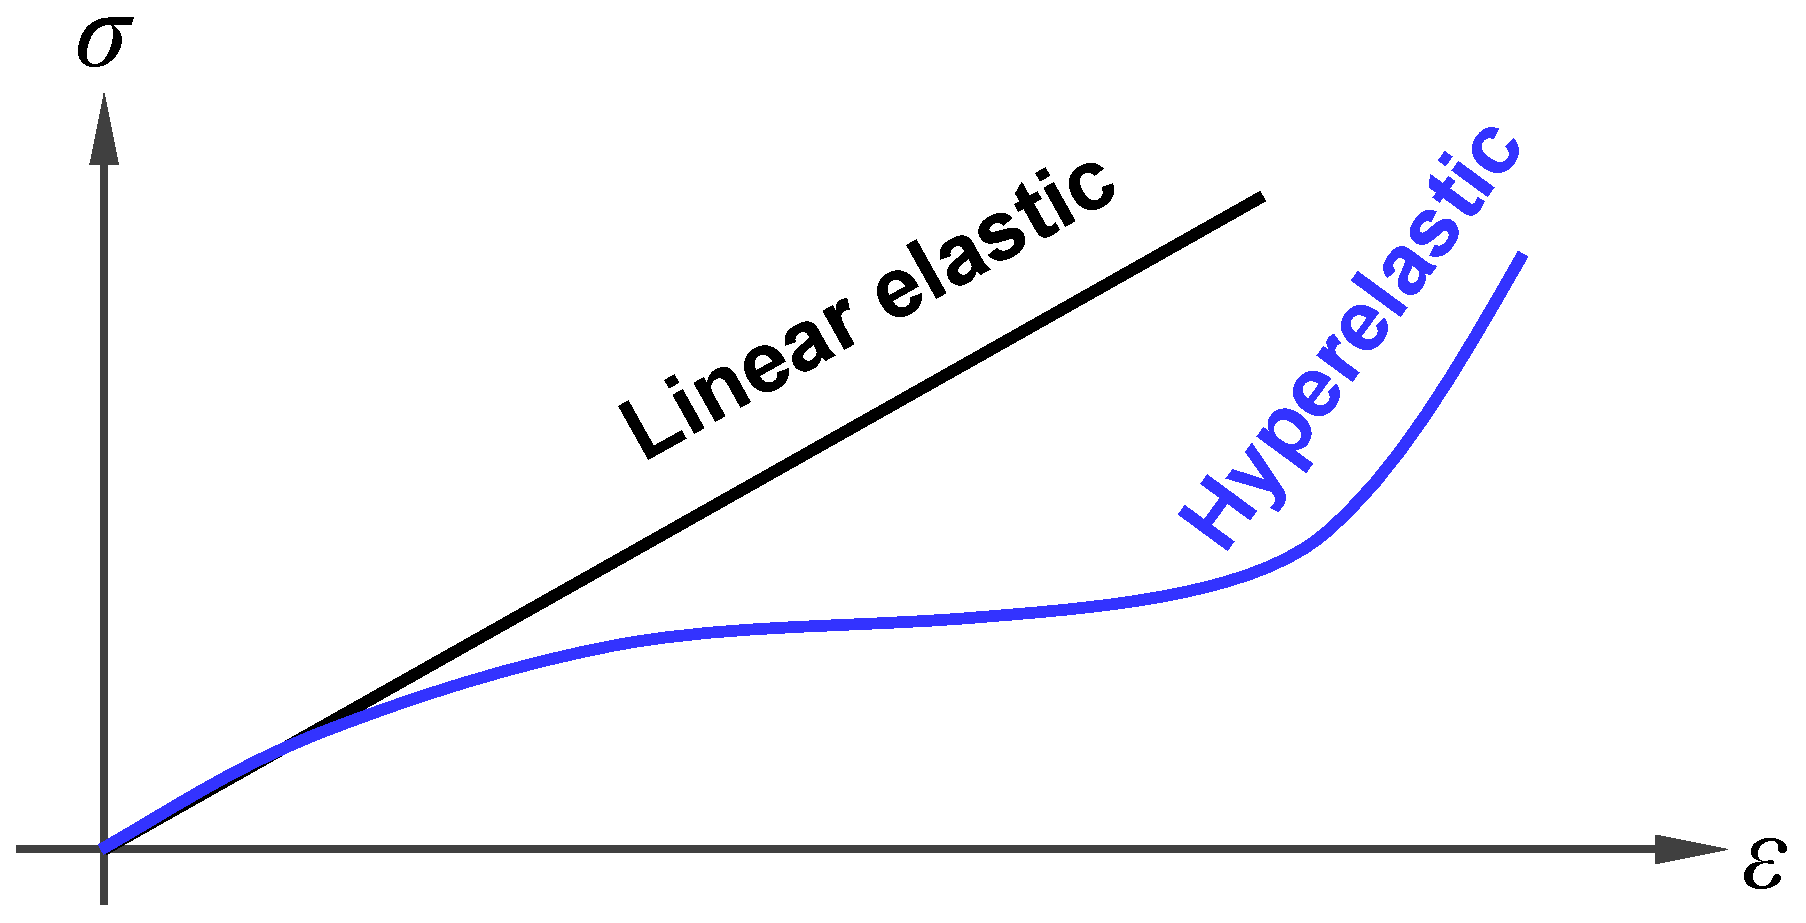
\includegraphics[width=0.5\linewidth]{figures/hyperelastic.eps}
    \caption{Hyperelastic tensile stress-strain curve showing nonlinear elastic behaviour compared with a linear elastic response}
    \label{fig:hyperelastic}
\end{figure}

Generally, hyperelastic materials are characterised by incompressibility ($J=1$, or $I_3^C=1$), where the volume is preserved during large deformations. Examples of hyperelastic materials are rubber and biological tissues. \\

Non-linear stress-strain relations can characterise hyperelastic materials, and this behaviour is often modelled using a strain energy density function, $W$. In this section, we first focus on the \textit{isotropic} hyperelastic material; in other words, the response of the material is identical regardless of the choice of the coordinate system. In order to achieve material frame indifference, the strain energy density functions are expressed using strain invariants of $\bf C$, \textit{i.e.}, $W(I_1, I_2, I_3)$.

\begin{table}[H]
\centering
\caption{Common hyperelastic strain energy functions}
\begin{tabular}{ll}
    \hline
    \textbf{Model} & \textbf{Strain energy function} \\
    \hline
    Neo-Hookean &
    $W = \frac{1}{2}\mu (I_1 - 3)$ \\[6pt]
    
    Mooney-Rivlin &
    $W = c_{10}(I_1 - 3) + c_{01}(I_2 - 3)$ \\[6pt]
    
    Yeoh &
    $W = c_{10}(I_1 - 3) + c_{20}(I_1 - 3)^2 + c_{30}(I_1 - 3)^3$ \\[6pt]
    
    Ogden &
    $W = \displaystyle\sum_{i=1}^{N} \frac{\mu_i}{\alpha_i}
    (\lambda_1^{\alpha_i} + \lambda_2^{\alpha_i} + \lambda_3^{\alpha_i} - 3)$ \\
    \hline
\end{tabular}
\label{tab:hyperelastic_models}
\end{table}

\end{document}